\documentclass[sigconf, screen]{acmart}

\usepackage{tabularx}
\usepackage[skins]{tcolorbox}
\usepackage{caption}
\usepackage{subcaption}
\usepackage{balance}

%%%%% Balance last page as requested by ACM Template %%%%%
\newcounter{BalanceAtReference}
\setcounter{BalanceAtReference}{52}
\newcounter{ReferenceIndexForBalancing}
\makeatletter
% Disable acmart's automatic invocation of \balance from \AtEndDocument,
% which is usually too late.
\global\@ACM@balancefalse
% Invoke command when the \bibitem reaches the specified value
\def\@balancelastpageonce{%
  \ifnum\value{ReferenceIndexForBalancing}=\value{BalanceAtReference}
    \balance
  \else
    \relax
  \fi
  \stepcounter{ReferenceIndexForBalancing}
}
\pretocmd{\bibitem}{\@balancelastpageonce}
  {} % on success
  {\@latex@error{Patching \bibitem failed}{\@ehd}}
\makeatother

\newcommand{\Code}[1]{\begin{small}\texttt{#1}\end{small}}
\newcommand*{\MyIndent}{\hspace*{0.3cm}}
\newcommand{\Tag}[1]{\tcbox[on line,boxsep=0pt,boxrule=0.2pt,left=3pt,right=3pt,top=3pt,bottom=3pt]{\begin{small}\textsf{#1}\end{small}}}

\tcbset{
  my box/.style={
    enhanced,
    colframe=#1!80,
    colback=#1!10,
    attach boxed title to top left={xshift=0.2cm, yshift=-0.2cm},
    boxed title style={
      colback=#1!80,
      outer arc=0pt,
      arc=0pt,
      top=0pt,
      bottom=0pt,
    },
  },
}
\newtcolorbox{result-rq}[1]{
  my box=black,
  title=#1,
  boxrule=1.2pt,top=6pt,bottom=3.5pt,left=6pt,right=6pt
}

\setcopyright{rightsretained}
\acmPrice{}
\acmDOI{10.1145/3468264.3468571}
\acmYear{2021}
\copyrightyear{2021}
\acmSubmissionID{fse21main-p271-p}
\acmISBN{978-1-4503-8562-6/21/08}
\acmConference[ESEC/FSE '21]{Proceedings of the 29th ACM Joint European Software Engineering Conference and Symposium on the Foundations of Software Engineering}{August 23--28, 2021}{Athens, Greece}
\acmBooktitle{Proceedings of the 29th ACM Joint European Software Engineering Conference and Symposium on the Foundations of Software Engineering (ESEC/FSE '21), August 23--28, 2021, Athens, Greece}

\begin{document}

\title{A Large-Scale Empirical Study on Java Library Migrations: Prevalence, Trends, and Rationales}

\author{Hao He}
% \orcid{0000-0001-8311-6559}
\affiliation{
  \institution{
    Department of Computer Science and
    Technology, Peking University, and Key Laboratory of High Confidence
    Software Technologies, Ministry of Education}
  \city{Beijing}
  \country{China}
}
\email{heh@pku.edu.cn}

\author{Runzhi He}
\affiliation{
  \institution{Department of Computer Science and
    Technology, Peking University, and Key Laboratory of High Confidence
    Software Technologies, Ministry of Education}
  \city{Beijing}
  \country{China}
}
\email{rzhe@pku.edu.cn}

\author{Haiqiao Gu}
\authornote{Works done at Peking University}
\affiliation{
  \institution{Department of Physics, Tsinghua University}
  \city{Beijing}
  \country{China}
}
\email{ghq17@mails.tsinghua.edu.cn}

\author{Minghui Zhou}
\authornote{Corresponding Author}
\affiliation{
  \institution{Department of Computer Science and
    Technology, Peking University, and Key Laboratory of High Confidence
    Software Technologies, Ministry of Education}
  \city{Beijing}
  \country{China}
}
\email{zhmh@pku.edu.cn}

%The rise of open-source software and package hosting platforms has led to an exponential growth of available 3rd-party libraries.
%Due to risks including security vulnerabilities, lack of maintenance, unexpected integration failures, or license issues, 
%Meantime, the adoption of 3rd-party libraries comes with various risks including, but not limited to security vulnerabilities, lack of maintenance, unexpected failures, and license issues.
%indicating the prevalence of library migrations. %% ***Note***: can we have ratio here? Because when people cite you, information in abstract is most important -- they may never bother to read the whole paper. And, is this info important: a median project with migrations has 2 to 4 migrations in total.
% We find that projects with library removals have one removal per 139 commits, and projects with migrations have 2 to 4 migrations in median.
%and most have no more than five migrations. %mostly among logging, JSON, testing, and web service libraries. 

\begin{abstract}

With the rise of open-source software and package hosting platforms, reusing 3rd-party libraries has become a common practice.
Due to various failures during software evolution, a project may remove a used library and replace it with another library, which we call \textit{library migration}.
Despite substantial research on dependency management, the understanding of how and why library migrations occur is still lacking.
Achieving this understanding may help practitioners optimize their library selection criteria, develop automated approaches to monitor dependencies, and provide migration suggestions for their libraries or software projects.
In this paper, through a fine-grained commit-level analysis of 19,652 Java GitHub projects, we extract the largest migration dataset to-date (1,194 migration rules, 3,163 migration commits).
We show that 8,065 (41.04\%) projects having at least one library removal, 1,564 (7.96\%, lower-bound) to 5,004 (25.46\%, upper-bound) projects have at least one migration, and a median project with migrations has 2 to 4 migrations in total. 
We discover that library migrations are dominated by several domains (logging, JSON, testing and web service) presenting a long tail distribution.
Also, migrations are highly unidirectional in that libraries are either mostly abandoned or mostly chosen in our project corpus. 
A thematic analysis on related commit messages, issues, and pull requests identifies 14 frequently mentioned migration reasons (e.g., lack of maintenance, usability, integration, etc), 7 of which are not discussed in previous work.
Our findings can be operationalized into actionable insights for package hosting platforms, project maintainers, and library developers.
We provide a replication package at \url{https://doi.org/10.5281/zenodo.4816752}.
\end{abstract}

\begin{CCSXML}
<ccs2012>
   <concept>
       <concept_id>10011007.10011006.10011072</concept_id>
       <concept_desc>Software and its engineering~Software libraries and repositories</concept_desc>
       <concept_significance>500</concept_significance>
       </concept>
   <concept>
       <concept_id>10011007.10011074.10011111.10011696</concept_id>
       <concept_desc>Software and its engineering~Maintaining software</concept_desc>
       <concept_significance>300</concept_significance>
       </concept>
   <concept>
       <concept_id>10011007.10011074.10011111.10011113</concept_id>
       <concept_desc>Software and its engineering~Software evolution</concept_desc>
       <concept_significance>300</concept_significance>
       </concept>
 </ccs2012>
\end{CCSXML}

\ccsdesc[500]{Software and its engineering~Software libraries and repositories}
\ccsdesc[300]{Software and its engineering~Maintaining software}
\ccsdesc[300]{Software and its engineering~Software evolution}

\keywords{library migration, mining software repositories, evolution and maintenance, empirical software engineering}

\maketitle

\section{Introduction}

Reusing existing 3rd-party libraries\footnote{
Developers use different terms interchangeably, such as libraries, packages, dependencies, components, frameworks, etc, to refer to a piece of reusable software (e.g. a JAR file~\cite{JAR}) available for download in a central hosting platform (e.g. Maven Central~\cite{Maven}). 
For consistency, we use the term ``library'' to refer to the reusable software itself, and the term ``dependency'' to emphasize that it is used by another software project.
} with ready-to-use features has long been a 
common practice in software development, which can increase software quality and development productivity~\cite{mohagheghi2007quality}.
Still, it is not until the rise of open-source software and the availability of central hosting platforms (e.g. Maven~\cite{Maven}, NPM~\cite{NPM}, PyPI~\cite{PyPI}, etc) in the recent decade that software reuse becomes so easy for both library users and library developers.
The number of newly published JARs on Maven Central has grown from 86,161 in 2010 to 364,218 in 2015 and 1,435,600 in 2020~\cite{Maven}.
As a result, 3rd-party libraries are widely adopted in both open-source and proprietary software projects, and a non-trivial software project often reuses dozens or even hundreds of existing libraries~\cite{thung2013automated, wang2020empirical}.

\begin{comment}
\begin{figure}[t]
    \centering
    \includegraphics[width=0.45\textwidth]{fig/growth.pdf}
    \caption{.}
    \label{fig:growth}
\end{figure}
\end{comment}

Meanwhile, the adoption of 3rd-party libraries brings unique challenges in the entire software life-cycle~\cite{cox2019surviving}.
First, given the wide spectrum of available libraries, even the task of choosing the right library for a specific purpose becomes non-trivial in which complex socio-technical factors need to be considered~\cite{pano2018factors, larios2020selecting}.
Second, increasing concerns are being raised about the risk of using outdated libraries as they may contain security vulnerabilities and unresolved issues~\cite{decan2018impact, pashchenko2018vulnerable, zimmermann2019small, alfadel2021empirical}, challenging the conventional strategy of ``if it ain't broke, don't fix it.''
Consequently, researchers study the characteristics, reasons, and drivers of library updates~\cite{bavota2015apache, kula2018developers, zerouali2018empirical} and practitioners propose industry solutions (e.g. Synk~\cite{Snyk}, WhiteSource~\cite{WhiteSource}, and GitHub Advisories~\cite{GitHubAdvisory}) that aim to keep libraries up-to-date and vulnerability-free. %%the last sentence doesn't have a predicate
However, failures or misalignment with a library inevitably happens and may not be resolvable by updating its version.
In such cases, the library has to be completely removed and replaced by another library, which are called \textit{library migration} in the literature~\cite{teyton2012mining, teyton2014study, kabinna2016logging, he2021multi, he2021migrationadvisor}. 

While a large body of existing researches are conducted to characterize and understand library adoption~\cite{pano2018factors, de2018empirical, kavaler2019tool, yin2020team, larios2020selecting, ma2020methodology, xu2020reinventing, lamba2020heard},
and library updates~\cite{cox2015measuring, kula2015trusting, bavota2015apache, mirhosseini2017can, kula2018developers, zerouali2018empirical, decan2018evolution, cogo2019empirical, soto2019emergence, dietrich2019dependency, zimmermann2019small}, 
researches on library migrations~\cite{bartolomei2009study, bartolomei2010swing, kabinna2016logging, alrubaye2020does, teyton2012mining, teyton2014study} are still %anecdotal, 
fragmented and incomplete.
%Existing studies are either experience reports~\cite{bartolomei2009study, bartolomei2010swing}, case studies~\cite{kabinna2016logging}, or large-scale mining studies with insufficient data~\cite{teyton2012mining, teyton2014study} for answering non-trivial questions.
More specifically, we lack understanding on: 1) how a large number of projects migrate their dependencies as a whole, and 2) what factors drive such migrations.
As the ultimate consequence of library adoption failures, such understanding will be a valuable source of information for developers, decision makers, and stakeholders.
It may help them optimize their library selection criteria, develop automated approaches to monitor dependencies, and provide migration suggestions for their libraries or software projects.
% It may also contribute to the general theory of technology transition~\cite{dosi1982technological, geels2002technological, smith2005governance, geels2007typology}, as an concrete example in the field of software engineering.
To bridge this knowledge gap, we seek to conduct a descriptive mixed methods study on large-scale open-source data to holistically understand how and why library migrations happen. More specifically, we ask the following research questions:
\begin{itemize}
    \item \textbf{RQ1:} How common are library migrations?
%    \begin{itemize}
%      \item \textbf{RQ1.1:} How frequently do projects remove a library? %%we can put these sub-questions to the results, where we start from splitting the questions with reasons explained in method section
%      \item \textbf{RQ1.2:} How frequently do projects migrate a library?
%    \end{itemize}
%   \item \textbf{RQ2:} How are library migrations conducted? 
    \item \textbf{RQ2:} How do migrations happen between libraries?
    \item \textbf{RQ3:} What are the frequently mentioned reasons when developers conduct a library migration?
    %\item \textbf{RQ3:} Can we use a predictive model to identify factors that lead to library migrations?
\end{itemize}

% 放在这里让这个表格出现在第二页
\begin{table*}
  \caption{Summary of Related Work on Library Migration}
\vspace{-1mm}
  \label{tab:related-work}
  \begin{tabularx}{\linewidth}{lp{48mm}p{30mm}p{62mm}}
  \toprule
    Paper & Subject of Study & Reported Prevalence & Reported Reasons \\
    \midrule
    Teyton et al.~\cite{teyton2012mining} & 80 migration rules & N.A. & convenience, outdated, incompatibilities\\
    Teyton et al.~\cite{teyton2014study} & 329 migration rules, 1,198 migrations, 26 commit messages & 5.57\% of 15,168 projects & feature, performance, configuration, bug, environment\\
    Kabinna et al.~\cite{kabinna2016logging} & 49 logging library migration attempts (33 successful) & 33 of 223 ASF projects (14.80\%) & feature, performance, flexibility, reduce future maintenance, reduce dependencies \\
    % Our Work & 3,215 migration commits & 9.95\% of 12,145 projects & deprecation, vulnerability, issue, feature, performance, usability, integration, maintenance, license, organization\\
  \bottomrule
  \end{tabularx}
% \vspace{-2mm}
\end{table*}

We face several challenges when answering these research questions.
First of all, the parallel and distributed nature of \Code{git}-based development presents unique peculiarities~\cite{bird2009promises} in an attempt to reconstruct accurate library change histories for a specific project.
Second, it is difficult to precisely define ``library migration'' and identify library migrations in commit history, while existing studies~\cite{teyton2012mining, teyton2014study} suffer from methodological limitations (details in Section~\ref{sec:background}).
To address these challenges, we propose an event-based dependency change model, formulate library migration based on dependency changes and self-admitted commit messages, retrieve migrations using a state-of-the-art mining algorithm~\cite{he2021multi}, and analyze migration frequency using upper-bound and lower-bound estimations.
By applying our method on 19,652 %Maven-managed 
Java projects and 4,022 libraries% on Maven Central
, we extract 2,629,992 dependency changes and 3,163 migration commits (the largest dataset compared with previous works in Table~\ref{tab:related-work}). 
We conduct exploratory data analysis for RQ1-2, and apply thematic analysis~\cite{cruzes2011recommended, braun2012thematic} to migration-related commits, issues, and pull requests to answer RQ3.
The key findings are:  %%%note, the contributions include both proposed methods and findings, e.g., Louvian community detection method is employed to detect library migration groups
\begin{enumerate}
    \item Both library removals and migrations are prevalent in the 19,652 Java projects, in which 8,065 have at least one library removal and 1,564 (lower-bound) to 5,004 (upper-bound) have at least one library migration. They are more likely to happen among projects with larger number of commits and dependencies. A median project with library removals has one removal per 139 commits and a median project with migrations has 2 to 4 migrations in total.
    % 44.07\% 8.98\% 28.72\%
    \item Library migrations from four domains (logging, testing, JSON, and web service) dominate the dataset, presenting a long tail distribution. And, migrations are highly unidirectional in that libraries within the same domain are either mostly abandoned or mostly adopted in the studied projects.
    \item Projects conduct library migrations for 14 different library-side and project-specific reasons. We identify 7 reasons not discussed in previous works. The most frequent reasons include lack of maintenance, feature, usability, integration with project context, and simplification of dependencies.
\end{enumerate}

Based on our findings, we summarize actionable insights for package hosting platforms, project maintainers, and library developers, including how to formulate and publicize best practices, how to select and integrate libraries, what to do with unmaintained libraries, and what to prioritize for library development.
We also identify aspects where current tooling support does not suffice and suggest future research directions. 

We provide a full replication package at Zenodo.\footnote{ \url{https://doi.org/10.5281/zenodo.4816752}} 
The scripts and documentation can also be accessed in this GitHub repository.\footnote{\url{https://github.com/hehao98/LibraryMigration}}

\section{Background and Related Work}
\label{sec:background}

Migration is a common phenomenon during software maintenance, which may refer to different development activities that stem from various motivations.
Common cases of migration include: migrating from one version to another version~\cite{kula2018developers}, one API to another API~\cite{alrubaye2019use}, one programming language to another programming language~\cite{zhong2010mining}, one platform to another platform~\cite{verhaeghe2019gui}, or one library to another library~\cite{teyton2012mining, teyton2014study, kabinna2016logging, he2021multi}.
In this paper, we use the term \textbf{library migration} to refer to the process of replacing one library with \textit{another}\footnote{More precisely, by \textit{another} we mean the \textit{names} (i.e., \texttt{groupId:artifactId} in Java) of the two libraries are different.} functionally similar or equivalent library. 
Given a library migration from library $l_1$ to library $l_2$, we refer to $l_1$ as the \textbf{source library}, $l_2$ as the \textbf{target library}, and $\langle l_1, l_2 \rangle$ as a \textbf{migration rule} in the subsequent paper.

Three steps are typically required for a library migration: justifying the necessity of a migration, finding the best target library, and modifying the code to use the new library.
For open-source projects, the first two steps are often facilitated through public discussions in issue trackers, where the benefits and costs are evaluated by developers~\cite{kabinna2016logging}.
Such discussions may not result in a migration if no consensus is reached or the perceived benefits do not outweigh the costs~\cite{kabinna2016logging}.
The cost mainly comes from the third step, which is known to be tedious, error-prone, and sometimes difficult~\cite{alrubaye2019use, chen2019mining}. % if the source library is deeply integrated
There are efforts that aim to improve development efficiency for the third step, by using API wrappers~\cite{bartolomei2009study, bartolomei2010swing}, mining API mappings~\cite{teyton2013automatic, alrubaye2019use, chen2019mining, alrubaye2020learning}, or directly editing code to use the new API~\cite{xu2019meditor, collie2020m3}. 
Studies also show that library migrations may improve code quality~\cite{alrubaye2020does}, but performance is rarely improved~\cite{kabinna2016logging}.

In this paper, we focus on understanding the first two steps of library migration, following existing studies~\cite{teyton2012mining, teyton2014study, kabinna2016logging} (Table~\ref{tab:related-work}). 
Teyton et al.~\cite{teyton2012mining} propose the concept of migration graph and a method to mine migration graph from software releases, where they get 80 migration rules and three reasons from real-world examples. 
In their subsequent study~\cite{teyton2014study}, they use a modified approach on the commit history of 15,168 projects and get 329 migration rules, 1,198 migrations and 26 commit messages that mentioned migration reasons.
Kabinna et al.~\cite{kabinna2016logging} analyze developer discussions of logging library migrations in Apache Software Foundation (ASF) projects, where they identify 49 migration attempts and five major reasons.
% However, the limited number of migrations obtained by Teyton et al.~\cite{teyton2012mining, teyton2014study} prevents them from deepening their results, while the results of Kabinna et al.~\cite{kabinna2016logging} may not generalize to other libraries.
However, the existing studies~\cite{teyton2012mining, teyton2014study, kabinna2016logging} have several limitations.
In particular, %Teyton et al.~\cite{teyton2012mining} only obtain a small number of migrations;
\cite{teyton2012mining} only obtain a small number of migrations;
%Teyton et al.~\cite{teyton2012mining, teyton2014study} 
\cite{teyton2012mining, teyton2014study} do not have a solid methodology foundation and are hard to reproduce. 
By their definition, a library migration happens if two libraries with similar functionalities co-exist and one gets removed in project history. 
The notion of ``similar'' is ambiguous and ``library migrations'' by this definition may be over-estimations. 
They also do not provide sufficient details about their manual identification criteria, nor do they share their dataset of library migrations.
Furthermore, %Teyton et al.~
\cite{teyton2014study} uses \textit{only} source code analysis for identifying libraries, which may miss migrations that only modify configuration files (e.g., migrate logger\footnote{\url{https://github.com/eclipse/leshan/commit/d103207}} or database\footnote{\url{https://github.com/mybatis/migrations-maven-plugin/commit/1b1c609}}). 
Finally, %Kabinna et al.~
\cite{kabinna2016logging} focuses %their study 
on a relatively small number (49) of \textit{logging} library migrations. Consequently, the findings in %Kabinna et al.~
\cite{kabinna2016logging} cannot reflect general trends and may not generalize to other kind of libraries.
%\begin{enumerate}
%    \item Teyton et al.~\cite{teyton2012mining} only obtain a small number of migrations.
%    \item Teyton et al.~\cite{teyton2012mining, teyton2014study} do not have a solid methodology foundation and are hard to reproduce. By their definition, a library migration happens if two libraries with similar functionalities co-exist and one gets removed in project history. The notion of ``similar'' is ambiguous and ``library migrations'' by this definition may be over-estimations. They also do not provide sufficient details about their manual identification criteria, nor do they share their dataset of library migrations.
    % We use a similar definition as upper-bound in RQ1 (Section~\ref{sec:rq1.2}) and the numbers are 3x larger than lower-bound. 
%    \item Teyton et al.~\cite{teyton2014study} use source code analysis for identifying libraries, which may miss migrations that only modify configuration files (e.g., migrate logger\footnote{\url{https://github.com/eclipse/leshan/commit/d103207}} or database\footnote{\url{https://github.com/mybatis/migrations-maven-plugin/commit/1b1c609}}). 
%    \item Kabinna et al.~\cite{kabinna2016logging} focus their study on a relatively small number (49) of \textit{logging} library migrations. Consequently, their findings cannot reflect general trends and may not generalize to other kind of libraries.
%\end{enumerate}
% Their limitations motivate us to conduct a new large-scale mining study to provide a comprehensive overview of how and why library migrations happen among a large number of projects and libraries.
%Therefore, we conduct a new study that mines 
In this study, we mine large-scale historical data to provide a comprehensive overview of how and why library migrations happen among a large number of projects and libraries.

Our work is also partially inspired by recent studies on library adoption~\cite{pano2018factors, de2018empirical, kavaler2019tool, yin2020team, larios2020selecting, ma2020methodology, lamba2020heard, xu2020reinventing} and library updates~\cite{cox2015measuring, kula2015trusting, bavota2015apache, mirhosseini2017can, kula2018developers, zerouali2018empirical, decan2018evolution, cogo2019empirical, soto2019emergence, dietrich2019dependency, zimmermann2019small}. 
In terms of library adoption, researchers use interviews and surveys to summarize developer considerations when choosing JavaScript frameworks~\cite{pano2018factors}, deciding whether to re-implement~\cite{xu2020reinventing}, and selecting libraries in general~\cite{larios2020selecting}.
Researchers also employ different modeling approaches to identify factors that lead to adoption between R dataframe libraries~\cite{ma2020methodology} and between JavaScript CI/CD tools~\cite{kavaler2019tool, yin2020team, lamba2020heard}. %%%"between a and b" but in different papers? should be two betweens
In terms of library update, researchers have investigated how developers update~\cite{bavota2015apache} or not update libraries~\cite{cox2015measuring, kula2015trusting, kula2018developers, soto2019emergence, zerouali2018empirical, decan2018evolution}, mechanisms to support library update~\cite{mirhosseini2017can, dietrich2019dependency}, and the impact of security vulnerabilities introduced by outdated libraries~\cite{zimmermann2019small, decan2018impact}.
However, they do not consider migrations between \textit{different} libraries, and our study can complement existing researches by providing findings about how previous library adoptions fail in projects and why developers choose to replace a library instead of updating it.
% Their findings indicate that library selection is non-trivial to get it right, but they do not consider the migrations between \textit{different} libraries, which can be used to observe how library selection fails.

\section{Data Collection}
\label{sec:data}

\subsection{Collecting Projects and Libraries}

We begin with the latest Libraries.io dataset~\cite{LibrariesIO} (released in Jan 2020), which is widely used in related research (e.g.~\cite{zerouali2018empirical, decan2019empirical, he2021multi, alfadel2021empirical}).
We choose to focus on Java projects because of Java's popularity and industrial importance, and because all previous works in this topic focus on Java~\cite{teyton2012mining, teyton2014study, kabinna2016logging}. %%so easy for comparison? looks like a different language is even better
We consider a repository on GitHub as a project and use the GitHub repository list in the dataset to select relevant repositories.
As a simple threshold for ensuring the quality of selected repositories, we select non-fork Java repositories with more than 10 stars, leaving us with 59,475 repositories.
We do not filter by the number of commits and recent activities % (e.g.~\cite{wang2020empirical})
because the goal of our study is to depict general longitudinal trends, not to observe the state-of-the-art practice by mature projects.
Then, to retrieve version control data for these projects, we use the World of Code database~\cite{ma2019world} (version R, constructed in April 2020). 
To simplify the task of dependency extraction, we focus on projects that use Maven~\cite{MavenTool} for build and dependency management.
These projects contain one or several configuration files named \Code{pom.xml} in their project paths, which has a \Code{<dependencies>} section where developers declare the group IDs, artifact IDs, and version numbers of required libraries.
The declarations are strict in that a build attempt will fail if a used library is not declared or included as a transitive dependency, but an unused library may still be declared, which is a threat to validity (Section~\ref{sec:threat-to-validity}).
By keeping repositories with at least one \Code{pom.xml} file in one of the repository's commits, we retain 19,652 repositories (23,988,437 commits in total).

The dependencies declared in project \Code{pom.xml} files may not fit the definition of a ``library,'' because they may be internal project modules not intended for reuse by other projects.
To filter out such cases, we only consider dependencies that 1) are accessible in Maven Central~\cite{Maven}, and 2) have been included in the \Code{pom.xml}s of more than 10 repositories in the aforementioned 19,652 repositories.
Finally, we get 4,022 libraries.\footnote{
Following general conventions, we consider a unique (group ID, artifact ID) pair as a library, and the version string for distinguishing different versions of a library.
% However, this definition does not consider library renames, which we will further discuss in the remainder of this section.
}
We sample 94 libraries (confidence level = 95\%, confidence interval = 10) and determine whether they are libraries or not by inspecting their descriptions in Maven Central and searching them on the Web. 
Ninety-three %93 
of 94 samples (98.93\%) contain public information indicating their appropriateness of reuse (e.g., terms such as library, framework, platform, specification, etc), which justifies our selection criteria.\footnote{
The only exception is \texttt{io.prometheus:simpleclient\_common} which describes itself as \textit{common code used by various modules of the \texttt{simpleclient}.}}

\subsection{Computing Dependency Changes}
\label{sec:depchg}

With projects and libraries collected, our next task is to extract dependency changes from project commit histories, as these dependency changes may indicate library migrations.
However, simply sorting and comparing all versions by time for a given \Code{pom.xml} file will generate too many false positives because a project may have many parallel branches which may or may not be merged, effectively forming a directed acyclic graph~\cite{bird2009promises} (DAG, see Figure~\ref{fig:gitdag}).
To take the DAG into consideration, we model each \textbf{dependency change} as an \textit{event} happened in one commit, which can be either an adoption, a removal, or a version change.
The event is computed from comparing with the prior \Code{pom.xml} file version in the parent commit.
More precisely, let commit $c_1$ be the parent of commit $c_2$, $L_1$ be the set of dependencies in \Code{pom.xml} file $f$ of commit $c_1$, and $L_2$ in file $f$ of commit $c_2$.
For $c_2$, the set of adoptions $D^+_{c_2}=L_2 - L_1$; the set of removals $D^-_{c_2}=L_1 - L_2$; and the set of version changes $D^v_{c_2} = \{ l \mid l \in L_1  \land l \in L_2 \land ver(l, c_1) \ne ver(l,c_2)\}$.
For $c_2$ in Figure~\ref{fig:gitdag}, $f=\text{\Code{tool/pom.xml}}$, $D_{c_2}^+=\{ \text{\Code{org.slf4j:slf4j-jdk14}}\}$, $D_{c_2}^-=\{ \text{\Code{log4j:log4j}} \}$, and $D_{c_2}^v=\{ \text{\Code{org.slf4j:slf4j-api}} \}$.
We ignore merge commits based on the assumption that merge commits are seldom used for making new changes other than conflict resolution.
To validate this assumption, we collect merge commits with \Code{pom.xml} diff from all repositories (207,553 in total, 8.2\% of all merge commits), and find that only 6,801 (3\%) have new dependency changes.
%\footnote{This assumption is widely used. For example, GitHub also excludes merge commits when counting the number of contributions and changed lines that a user made. } %%what is the proportion of this kind of commits? Hao: Can't answer because it is not detectable
Through an iteration over all commit diffs of all projects, we get 2,629,992 dependency changes from 302,774 commits.

\begin{figure}[t]
  \centering
  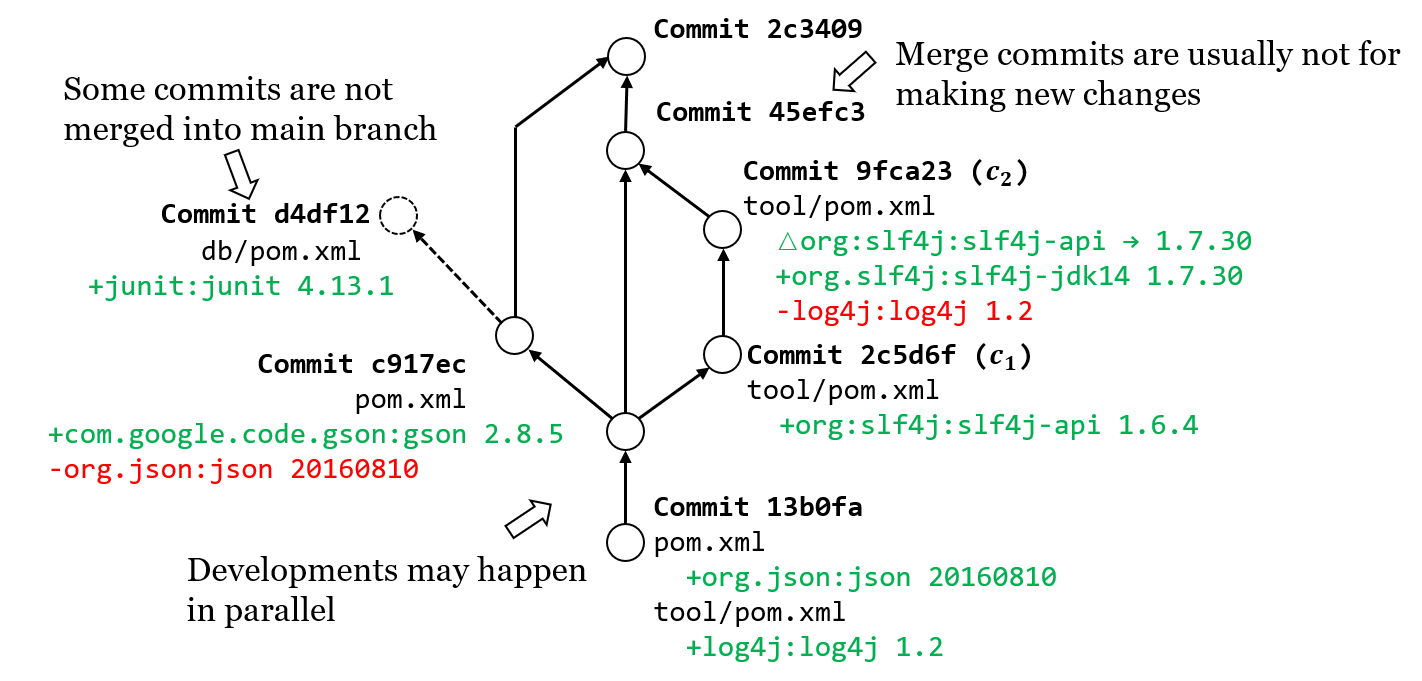
\includegraphics[width=0.9\linewidth]{fig/git-dag.png}
\vspace{-3mm}
  \caption{An example project commit history.}
  \label{fig:gitdag}
\vspace{-2mm}
\end{figure}

\subsection{Identifying Library Migrations}
\label{sec:get-lib-mig}

\begin{table}
  \caption{Statistics of the Collected Dataset}
\vspace{-3mm}
  \label{tab:data}
  \begin{tabular}{ll}
  \toprule
    Data & Size/Statistics \\
    \midrule
    Projects ($\mathcal{P}$) & 19,652 \\
    \MyIndent Stars                    & \MyIndent median = 32, stddev = 1407.93\\
    \MyIndent Commits                  & \MyIndent median = 142, stddev = 5614.70 \\
    \MyIndent Active Months            & \MyIndent median = 27, stddev = 26.97 \\
    \MyIndent \Code{pom.xml} Files     & \MyIndent median = 2, stddev = 75.72 \\
    Libraries ($\mathcal{L}$)          & 4,022 \\
    \MyIndent Versions                 & \MyIndent median = 26, stddev = 104.20\\
    \MyIndent Included Repositories    & \MyIndent median = 25, stddev = 310.94\\
    Dependency Changes ($\mathcal{D}$) & 2,629,992 (302,774 commits) \\
    \MyIndent Adoptions ($\mathcal{D}^+$) & \MyIndent 1,771,664 (208,691 commits)\\
    \MyIndent Removals ($\mathcal{D}^-$) & \MyIndent 290,150 (56,377 commits)\\
    \MyIndent Version Changes ($\mathcal{D}^v$) & \MyIndent 568,178 (97,447 commits)\\
    Migration Rules ($\mathcal{R}$)    & 1,194 (393 renames) \\
    Migration Commits ($\mathcal{M}$)  & 3,163 (1,459 renames) \\
  \bottomrule
  \end{tabular}
\vspace{-4mm}
\end{table}

The dependency changes we collected before may not be necessarily related to a library migration, but it is non-trivial to define and identify real library migrations from dependency changes.
First, we need to determine whether a migration is feasible between two arbitrary library pairs (i.e., for $l_1$ and $l_2$, whether $\langle l_1, l_2 \rangle$ is a migration rule).
Next, we need to identify commits related to a library migration.
To deal with these challenges, we define a commit as a \textbf{migration commit} when its commit message clearly indicates a migration (e.g. \textit{Replace org.json with jackson}~\cite{Commit-replace-json}), and define $\langle l_1, l_2 \rangle$ as a \textbf{migration rule} if and only if we can find a migration commit that conducted the migration from $l_1$ to $l_2$.

We acquire migration commits and migration rules from the dependency changes using a state-of-art mining algorithm~\cite{he2021multi} and manually validate the returned results.
%\footnote{A brief description of the validation procedure is available in the anonymized GitHub repository for this paper (see Introduction)}
For each source library query, the algorithm mines possible target libraries, %from \textit{all} libraries in Maven Central, 
rank each target library by a confidence value, and returns possible migration commits from the source library to the target library based on the collected dependency changes.
However, it generates a tremendous amount of output if we query using all the 4,022 libraries.
To reduce human inspection effort, we use a combination of 1) source libraries provided in~\cite{teyton2012mining}, 2) 500 most popular libraries by number of adoptions in our repository dataset, as the query to the algorithm (670 queries in total).
For the output of each query, we focus on inspecting the returned commits for target libraries that have non-zero confidence value, rank top-20 among all returned target libraries, and exist in the aforementioned 4,022 libraries.
After validation, we obtain 1,194 migration rules (390 source libraries, 562 target libraries) and 3,163 migration commits.
We obtain the largest dataset compared with previous work (Table~\ref{tab:related-work}), but the size of migration commits by this definition is doomed to be small because most commits do not have informative commit messages~\cite{cortes2014automatically}.
% Second, to reduce human labeling effort, we only validate results that the algorithm consider them likely to be correct~\cite{he2021multi}.
Thus, this set of migrations can only be viewed as a \textit{subset} of real world migrations
%Although they can only be used to compute a lower-bound estimation 
and inadequate for answering migration popularity (RQ1), but they are guaranteed to be correct and invaluable for unveiling migration behavior (RQ2) and reasons for migration (RQ3).

Some migrations happen because of a library \textit{rename}, which often accompanies important library changes (e.g., major version update, license change, organization switch, etc) and falls near the boundary of library update and library migration.
We detect these rules by finding all rules whose artifact IDs contain overlapping terms (excluding terms like \Code{api}, \Code{core}, \Code{all}, etc) and manually validating the results, resulting in 393 \textbf{rename rules}.
Teyton et al.~\cite{teyton2014study} exclude rename rules by manually mapping \Code{groupId:artifactId} to "library names."
However, library renames are 1) very common at least in Java/Maven, 2) developers also state them as migrations in commit messages, and 3) their APIs are often significantly reworked. 
Thus, we choose to retain rename rules in subsequent analysis as a special type of migration rule, and distinguish them from other rules where their property significantly differs.

In the remainder of this paper, we denote $\mathcal{P}$ as the set of repositories (i.e., projects), $\mathcal{L}$ as the set of libraries, $\mathcal{D}$ as the set of dependency changes ($\mathcal{D}^+, \mathcal{D}^-, \mathcal{D}^v$ for adoption, removal and version changes, respectively), $\mathcal{R}$ as the set of migration rules, and $\mathcal{M}$ as the set of migration commits. The statistics of collected data are summarized in Table~\ref{tab:data}.

\section{RQ1: How common are library migrations?}
%%% explain we split this question with two sub-questions because ..... ok, u had explanation for each sub-question. u can move them here, so we know what to expect from the very beginning with a big picture

Since library migration is the process of removing a library and introducing another library, a library removal and a library adoption are \textit{necessary} for a library migration.
To the best of our knowledge, library removals during software evolution have never been studied before.
Intuitively, %a large part of library removals should lead to library migrations, 
if many projects remove a library, it is probably followed by migrations,
and
it is unknown exactly how many removals are related to migrations and how migrations are distributed in our project corpus.
Thus, we ask two sub-RQs:

\textbf{RQ1.1:} How frequently do projects remove a library?

\textbf{RQ1.2:} How frequently do projects migrate a library? 

\subsection{RQ1.1: Removal Frequency Analysis}

\subsubsection{Methodology}

We consider all types of dependency changes during analysis for comparison purposes.
For project $p \in \mathcal{P}$, let $C_p$ be the set of commits for $p$, $D_p$ be the set of dependency changes happened in $p$ (i.e., $D_p=\bigcup_{c \in C_p}D_c$).
We first consider projects $P_r \subset \mathcal{P}$ with at least one removal, i.e., $P_r=\{p \mid p\in \mathcal{P} \land D_p^- \ne \emptyset\}$, and analyze its distribution within $\mathcal{P}$.
Then, for $p\in P_r$, we compute and compare the distributions for 1) the number of changes in project $p$ for all change types (i.e., $\sum_{c \in C_p} |D|$ for $D \in \{D_c, D_c^+, D_c^-, D_c^v\}$), and 2) the average number of commits between changes for all change types (i.e.,  $|C_p| / |\{c \mid c \in C_p \land D \ne \emptyset\}|$ for $D \in \{D_c, D_c^+, D_c^-, D_c^v\}$).
We use the latter to estimate the frequency (or interval) of each change type along the project development history.
%As an additional metric, we compute retention rates for projects, defined as follows
%\begin{align}
    %Retention(p) &= 1 - |D_p^-| / |D_p^+|, p \in P_r
    %Retention(l) &= 1 - |\{l | \langle l, v \rangle \in \mathcal{D}^-\}| / |\{l | \langle l, v \rangle \in \mathcal{D}^+\}|, l \in \mathcal{L}
%\end{align}

\subsubsection{Results}

\begin{figure}[t]
  \centering
  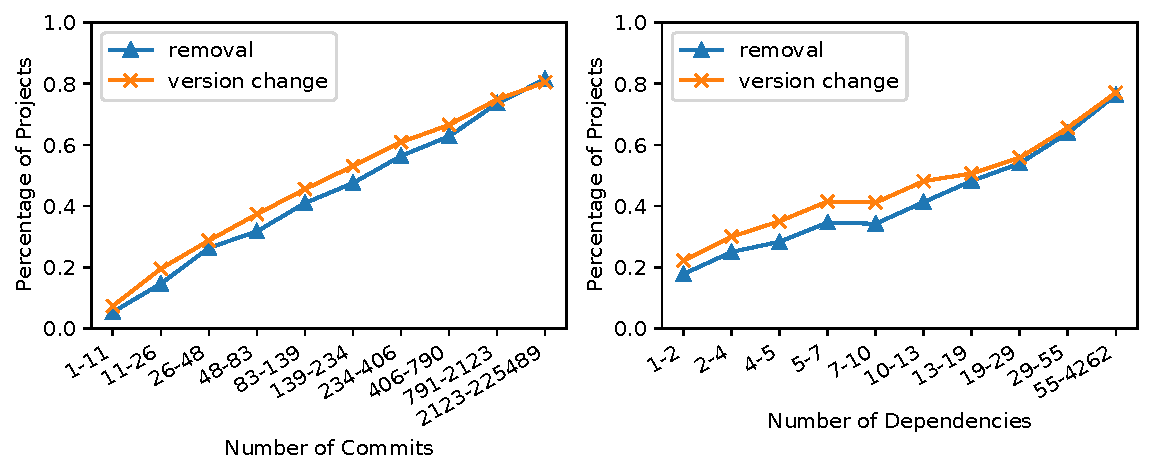
\includegraphics[width=\linewidth]{fig/chgrel.pdf}
\vspace{-7mm}
  \caption{Distribution of $P_r$ by number of commits / dependencies, with that of $P_v=\{p|p\in \mathcal{P} \land D_p^v \ne \emptyset\}$ for comparison.}
  \label{fig:chgrel}
\vspace{-4mm}
\end{figure}

For all 19,652 projects ($\mathcal{P}$), 1398 (7.11\%) projects do not have any dependency changes because their \Code{pom.xml} files have no or empty \Code{<dependencies>} sections. 
Among the remaining 18,254 projects, 8,657 (47.43\%) have at least one version change and 8,045 (44.07\%) have at least one removal.
The two major reasons for not having any removals or version changes are that, these projects do not have sufficient development histories or only have a few number of dependencies.
By dividing the 18,254 projects into 10 equally sized chunks separated by number of commits, we show on the left side of Figure~\ref{fig:chgrel} that migrations are more likely to happen in projects with higher number of commits, and the trend is very similar to that of version changes. % with slightly lower frequencies.
A Spearman correlation test between number of removals and number of commits for all projects yields a coefficient $\rho$ of $0.532$ ($p < 0.001$), which indicates moderate to strong correlation.
A similar trend can be observed for number of dependencies on the right side of Figure~\ref{fig:chgrel}, but the correlation is weaker ($\rho = 0.158$, $p < 0.001$).

For the 8,045 projects with at least one removal ($P_r$), we plot the distribution of the number of changes and the average number of commits between changes for all change types in Figure~\ref{fig:chgdis}.
Among $P_r$, a median project has 35 adoptions, 6 removals, 6 version changes, one adoption per 48 commits, one removal per 139 commits, and one version change per 167 commits.
The variations are also high across different projects, with version changes having higher variance than removals.
%In terms of retention rates, a median project in $P_r$ only retain 80.00\% of its adopted libraries (mean = 73.31\%, stddev = 22.42\%) until our last observation.
%while a median library can only retain 80.39\% of its users (mean = 76.46\%, stddev = 16.09\%). 
We conclude that apart from library updates and adoptions, library removals are also very common for these projects.


\begin{figure}[t]
  \centering
  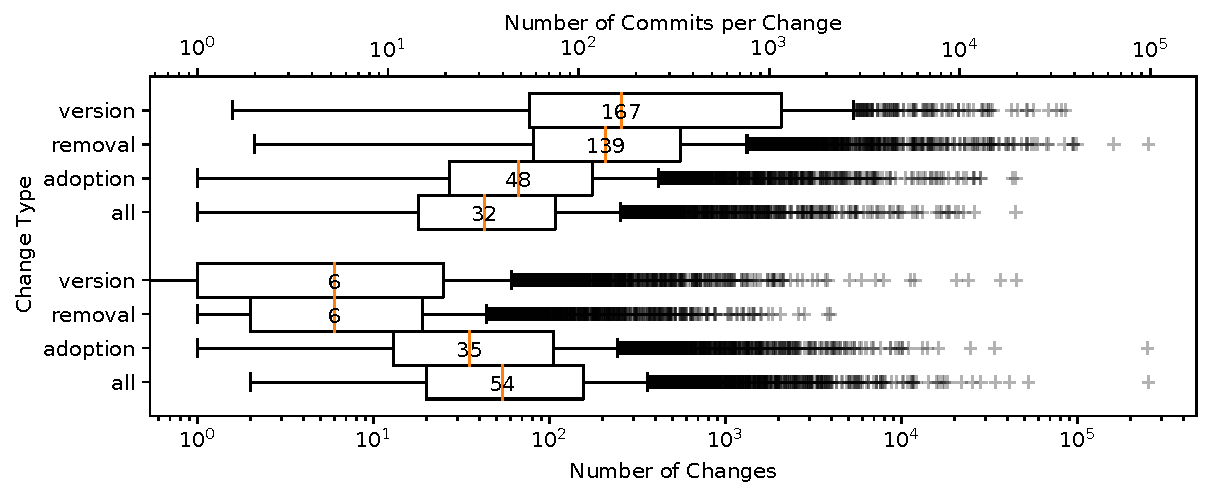
\includegraphics[width=\linewidth]{fig/chgdis.pdf}
\vspace{-7mm}
  \caption{
   Distribution of the number of changes (below) and the average number of commits between changes (above).
  %Distribution of $\sum_{c \in C_p} |D|$ (below) and $|C_p| / |\{c|c \in C_p \land D \ne \emptyset\}|$  (above) for $D \in \{D_c, D_c^+, D_c^-, D_c^v\}$, $p \in P_r$.
  }
  \label{fig:chgdis}
\vspace{-4mm}
\end{figure}

\begin{comment}
\begin{figure}[t]
  \centering
  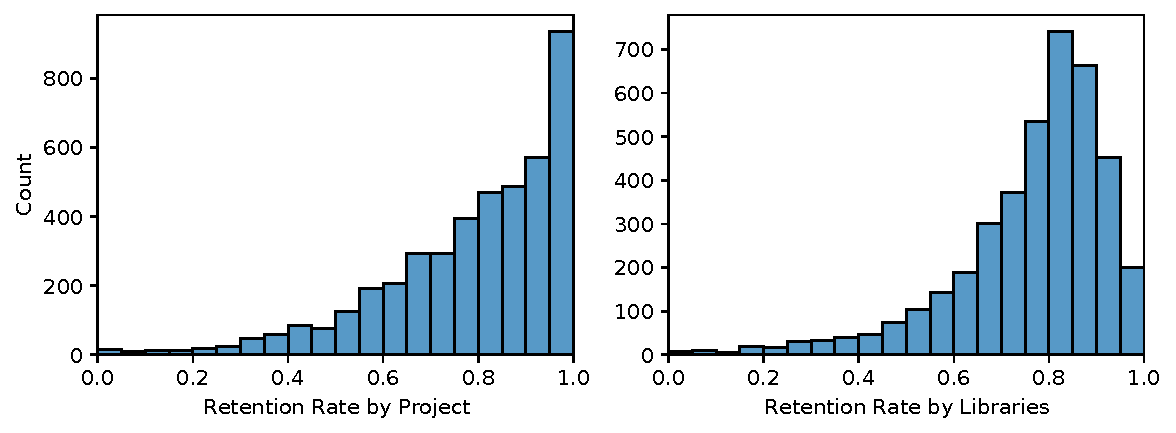
\includegraphics[width=0.95\linewidth]{fig/retention.pdf}
\vspace{-3mm}
  \caption{Distribution of $Retention(p)$ and $Retention(l)$.}
  \label{fig:retention}
\vspace{-2mm}
\end{figure}
\end{comment}

\begin{result-rq}{Summary for RQ1.1:}
Among projects with dependencies, 44.07\% have at least one library removal.
%Library removals are common during software evolution for a large part of software projects.
%For those projects, removal frequency is similar to update frequency. %i thought update frequency == migration frequency?
For those projects, a median project has one removal per 139 commits (for comparison, one version change per 167 commits).
Removals are more likely to happen for projects with higher number of commits and dependencies.
%In general there is one adoption per 48 commits, one removal per 139 commits in median.
\end{result-rq}

\subsection{RQ1.2: Migration Frequency Analysis}
\label{sec:rq1.2}

%\subsubsection{Motivation}

%The results of RQ1.1 have demonstrated the prevalence of library removals in Java OSS projects.
%Based on the intuition that a large part of library removals should lead to library migrations, we hypothesize that library migrations are also likely to be prevalent in our project corpus.
%However, it is still unknown exactly how many removals are related to library migrations and how library migrations are distributed in our project corpus, so we ask \textbf{RQ1.2:} How frequently do projects migrate a library? 

\subsubsection{Methodology}

We begin with $\mathcal{M}$ and $\mathcal{R}$ mentioned in Section~\ref{sec:get-lib-mig}, which contains 716 libraries (denote as $L_m \subset \mathcal{L}$).
By limiting our analysis on projects that have once adopted any of these libraries, we obtain 17,426 projects and denote as $P_m = \{p \mid p \in \mathcal{P} \land \exists l,\ l \in L_m \land l \in D_p^+\}$.

The computation of frequency for library migrations is difficult because we cannot guarantee the completeness of mined migrations for any non-trivial mining approach~\cite{teyton2012mining, he2021multi}.
As mentioned in Section~\ref{sec:get-lib-mig}, $\mathcal{M}$ and $\mathcal{R}$ are subsets of real world migration commits and migration rules, which can only be used to estimate lower-bound frequencies.
We refer to such cases as \textbf{confirmed migrations} in this section and denote $P_{cm}\subset \mathcal{P}$ as the set of projects with at least one confirmed migration.
As an upper-bound estimation, we propose it is likely that $p$ has also conducted the same migration if $\langle l_1, l_2 \rangle$ is a migration rule and $l_1$ is removed and $l_2$ is added in a \Code{pom.xml} file of project $p$.
More formally, let $D_{p,f}$ be the set of dependency changes happened in \Code{pom.xml} file $f$ of project $p$, we hypothesize that if $\langle l_1, l_2 \rangle \in \mathcal{R} \land l_1\in D_{p,f}^- \land l_2 \in D_{p,f}^+$, a library migration may have happened in $f$ of $p$.
Similar to $P_{cm}$, we refer to such cases as \textbf{possible migrations} and denote $P_{pm} \subset \mathcal{P}$ as the set of projects with at least one possible migration.

Similar to RQ1, we first analyze the distribution of $P_{cm}$ and $P_{pm}$ within $P_m$ and its relationship with number of commits and number of dependencies.
Then, we analyze the distribution of library migrations within $P_{cm}$ and $P_{pm}$.
For each project $p$, we count the number of migrations by the number of migration rules to avoid duplication when a project simultaneously performs the same migration in many \Code{pom.xml} files, or in different branches in which some may not be merged.
More formally, we define
\begin{equation}
\label{eq:migcount}
   MigCnt(p) = |\{\langle l_1,l_2 \rangle \mid \langle l_1, l_2 \rangle \in \mathcal{R} \land l_1 \in D_{p,f}^- \land l_2 \in D_{p,f}^+\}|
\end{equation}
Finally, for each migration commit $m \in \mathcal{M}$, we use its commit timestamp to plot a longitudinal trend of library migrations.

\subsubsection{Results}

\begin{figure}[t]
  \centering
  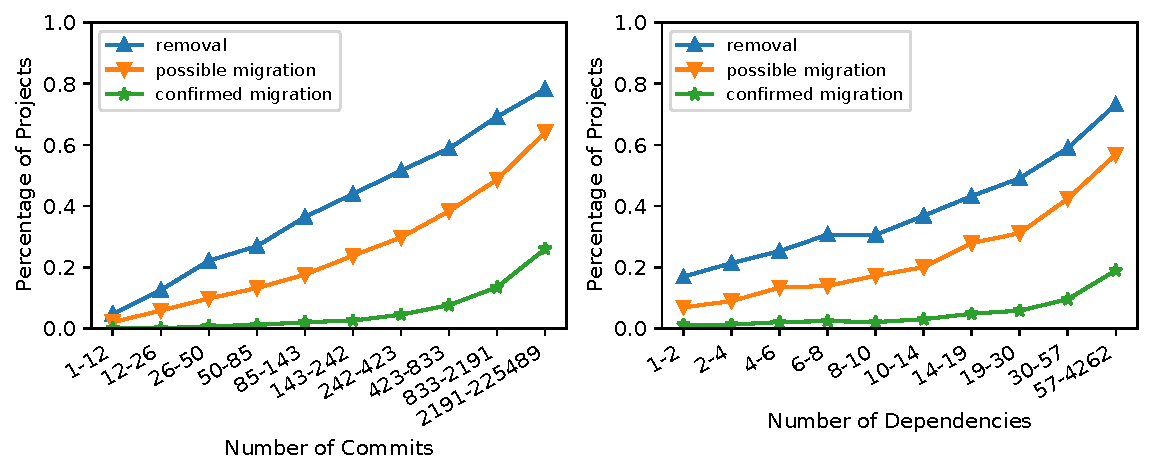
\includegraphics[width=\linewidth]{fig/migrel.pdf}
\vspace{-7mm}
  \caption{Distribution of $P_{cm}$ and $P_{pm}$ by number of commits and dependencies. We also show the results of $P_r'=\{p|p\in P_m \land D_p^- \ne \emptyset\}$ for comparison.}
  \label{fig:migrel}
\vspace{-4mm}
\end{figure}

Among the 17,426 projects ($P_m$), 7,950 (45.62\%) have at least one removal of libraries in $L_m$, 5,004 (28.72\%) projects have at least one possible migration ($P_{pm}$), and 1,564 (8.98\%) projects have at least one confirmed migration ($P_{cm})$.
As a rough estimation, up to 62.94\% (5,004 / 7,950) of the projects have removals that lead to a library migration, for 31.25\% (1,564 / 5,004) of  which we can confirm in commit messages.
% For migration frequency, even the lower-bound estimation of 8.98\% is higher than the reported prevalence in Teyton et al.~\cite{teyton2014study} (see Table~\ref{tab:related-work}), indicating that library migrations have become more prevalent since their publication.
Although library migrations may not be very common in $P_m$ which contains projects with few commits or few dependencies, we show that library migrations are much more common for projects with many commits and dependencies (Figure~\ref{fig:migrel}) ($\rho=0.456$, $p < 0.001$ for commits, and $\rho=0.075$, $p<0.001$ for dependencies using Spearman correlation test).
Among the 3,796 projects with more than 10 dependencies and 143 commits (both are median values in $P_m$), 2,161 (56.93\%) / 764 (20.13\%) projects have at least one possible / confirmed migration.
Furthermore, we plot the distribution of projects by number of migrations happened in $P_{pm}$ and $P_{cm}$ (Figure~\ref{fig:migdist}).
As expected, their distributions resemble the shape of a long-tail distribution, where most projects have one or a few migrations and some projects have many more. 
A median project in $P_{pm}$ has undergone 4 possible migrations (mean = 9.33, stddev = 17.30, max = 337) and a median project in $P_{cm}$ has undergone 2 confirmed migrations (mean = 3.35, stddev = 4.54, max = 46).
Although there are extreme cases, the majority of projects (61.59\%$\sim$84.78\%) have no more than five migrations.
Finally, Figure~\ref{fig:migyear} shows the number of migration commits in each year, and we can observe a clear increasing trend (note that we only have partial data for 2020). 
This indicates that library migrations are becoming increasingly prevalent in the Java/Maven ecosystem since the publication of Teyton et al.~\cite{teyton2014study}.

\begin{figure}[t]
  \centering
  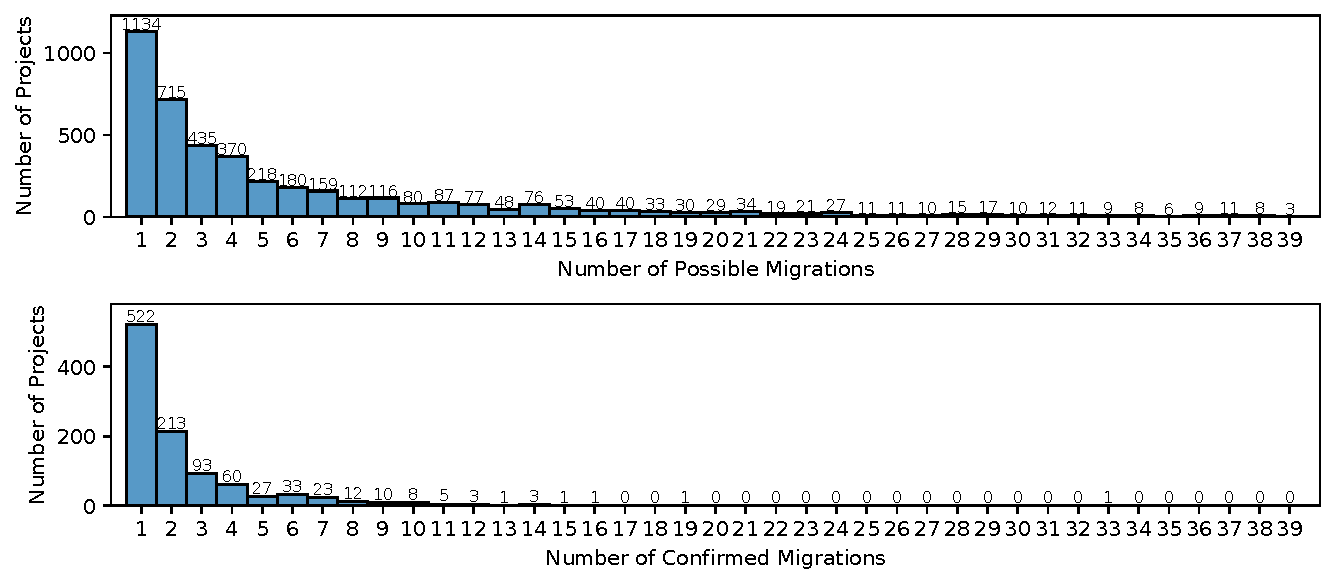
\includegraphics[width=\linewidth]{fig/migdist.pdf}
\vspace{-7mm}
  \caption{Distribution of projects by number of migrations.}
  \label{fig:migdist}
\vspace{-4mm}
\end{figure}

\begin{figure}[t]
  \centering
  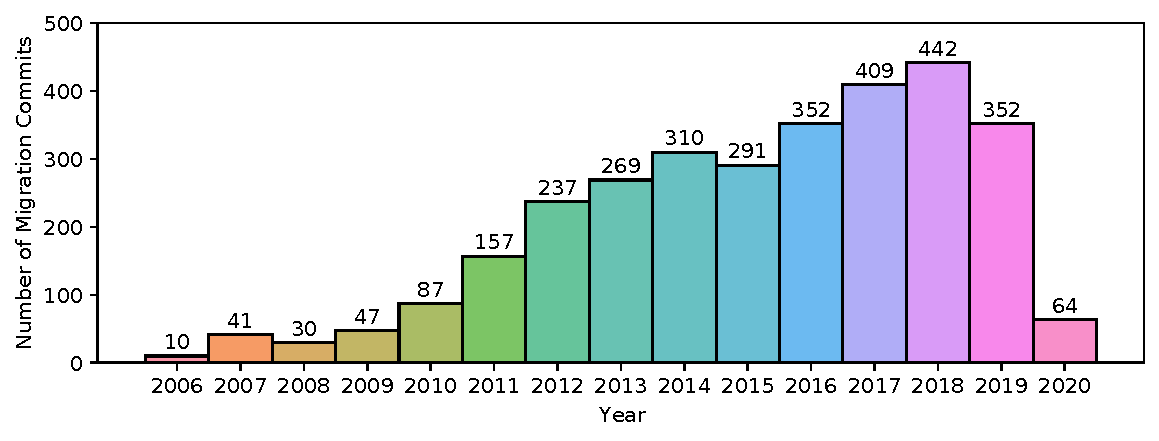
\includegraphics[width=\linewidth]{fig/migyear.pdf}
\vspace{-7mm}
  \caption{Number of migration commits in each year.}
  \label{fig:migyear}
\vspace{-4mm}
\end{figure}

\begin{result-rq}{Summary for RQ1.2:}
In the studied project corpus, 8.98\% to 28.72\% have undergone at least one library migration.
For those projects, most have no more than five migrations.
The probability of undergoing a library migration becomes significantly higher for projects with larger number of commits and dependencies.
\end{result-rq}

\section{RQ2: How do migrations happen between libraries?}

The results of RQ1 have demonstrated that library migrations have happened in a significant number of software projects.
However, it is still unclear how exactly library migrations are conducted, in particular, what kind of migrations are performed, among what kind of libraries, and whether or not the migrations share common behavior. %%need to tie the results to the questions. %%results: Library migrations are highly unidirectional in that most libraries are either mostly adopted or mostly abandoned.
%To bridge this knowledge gap, we seek to perform analysis on migration related libraries to answer \textbf{RQ2:} What is the general trend of library migrations?
Therefore, we ask \textbf{RQ2:} How do migrations happen between libraries?

\subsection{Methodology}

We adopt the concept of \textbf{migration graph} proposed by Teyton et al.~\cite{teyton2012mining, teyton2014study} as the basis to facilitate further analysis.
We define the migration graph in our study as a weighted directed graph $\langle L_m, \mathcal{R}, w \rangle$, where libraries in $L_m$ are nodes, migration rules in $\mathcal{R}$ are edges, and $w()$ is an edge weighting function.
For $\langle l_1, l_2 \rangle \in \mathcal{R}$, we compute weight $w(l_1, l_2)$ by counting the number of projects that have performed a migration from $l_1$ to $l_2$ in $\mathcal{M}$.

To demonstrate the extent to which a library is more likely to be a migration source or a migration target, we define the following metric $flow(l)$ for library $l \in L_m$
\begin{equation}
    flow(l) = \frac{deg^-(l) - deg^+(l)}{deg^-(l) + deg^+(l)}
\end{equation}
where $deg^-(l)$ is the weighted indegree for node $l$ and $deg^+(l)$ is the weighted outdegree for node $l$. 
Obviously, $flow(l) \in [-1, 1]$, where $flow(l) = 1$ means $l$ is always a target library and $flow(l) = -1$ means $l$ is always a source library.

To understand what kind of migrations are performed and to effectively visualize the graph, we divide migration rules into different application domains. 
First, we use Louvain community detection~\cite{blondel2008fast} on the migration graph to get 116 initial clusters.
Then, we use library descriptions, labels in Maven Central, and information from search engines to merge clusters, resolve cluster names, and correct errors.
The application domain of each migration rule $(l_1, l_2)$ is assigned from the domain of $l_1$ and $l_2$ when the two libraries are in the same domain, which is the case for 1,055 rules (88.44\%).
For the remaining rules, $l_1$ and $l_2$ fall into different domains either because the boundaries between domains is sometimes unclear or migrations can happen between different domains (e.g. from a XML library to a JSON library for serialization).
We get 53 application domains in total, among which 16 domains have more than 10 migration rules. 
The domain distribution is shown in Figure~\ref{fig:migcat}.
Four domains (web service, logging, JSON, and testing) dominate the dataset with 648 migration rules (61.42\%).
If we count the number of migrations happened (Figure~\ref{fig:migrepodist}), migrations between logging libraries and JSON libraries happen 1.4-1.7x more than testing and web service libraries.
Finally, we visualize sub-graphs for important application domains using Sankey diagrams~\cite{riehmann2005interactive}, which are often used to visualize how things flow in complex networks.
%in which libraries with $flow(l) \le 0$ are on the left side and libraries with $flow(l) > 0$ are on the right side.

\subsection{Results}

\begin{figure}
  \centering
  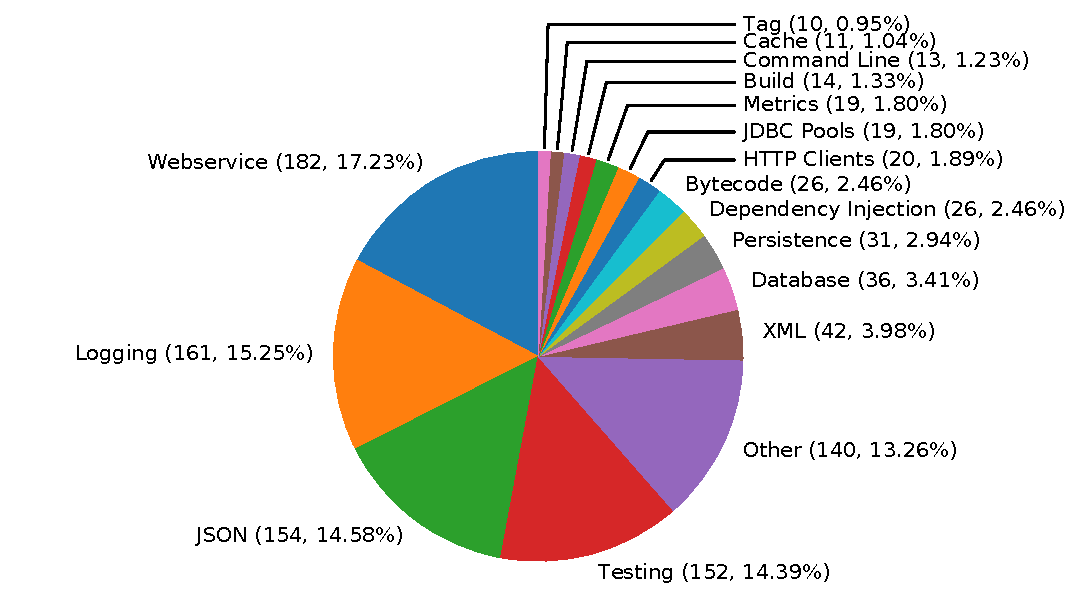
\includegraphics[width=\linewidth]{fig/migcat.pdf}
  \vspace{-6mm}
  \caption{Distribution of $\mathcal{R}$ by application domain.}
  \label{fig:migcat}
  \vspace{-4mm}
\end{figure}

\begin{figure}
  \centering
  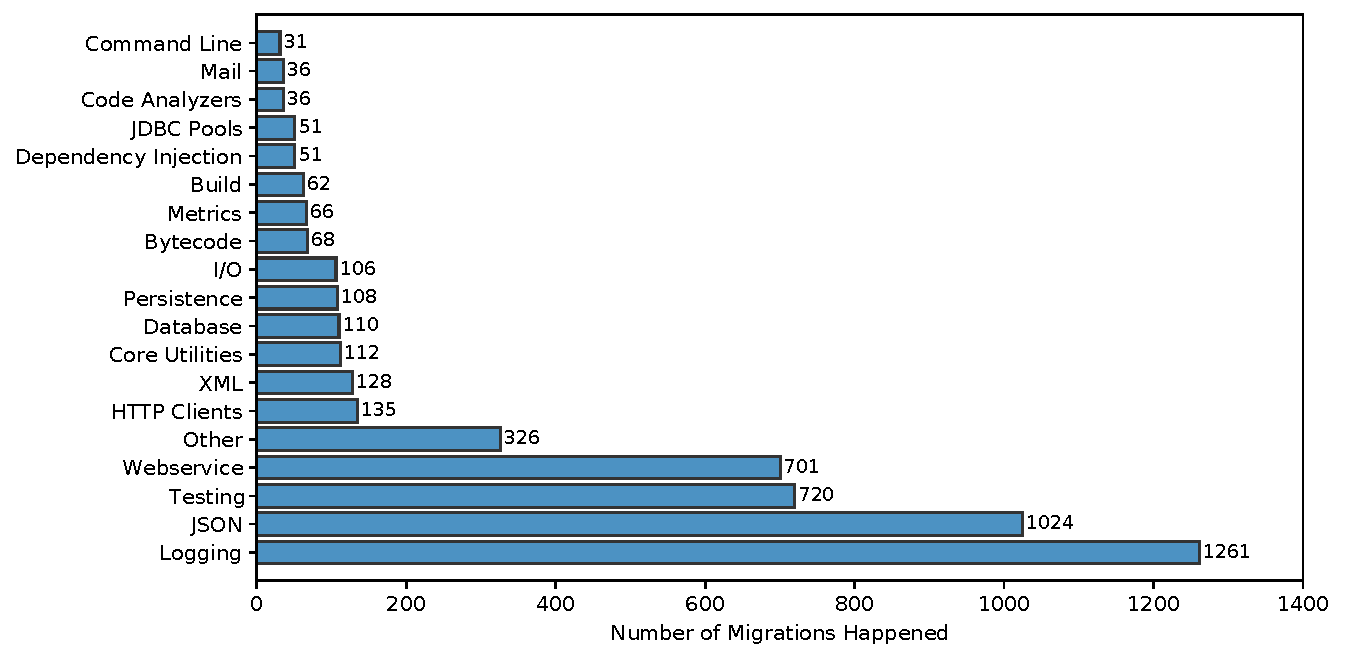
\includegraphics[width=\linewidth]{fig/migrepodist.pdf}
  \vspace{-6mm}
  \caption{Number of migrations for migration rules in each application domain ($\sum_{p\in \mathcal{P}} MigCnt(p)$, Equation \ref{eq:migcount}).}
  \label{fig:migrepodist}
  \vspace{-4mm}
\end{figure}

\begin{figure}
\centering
  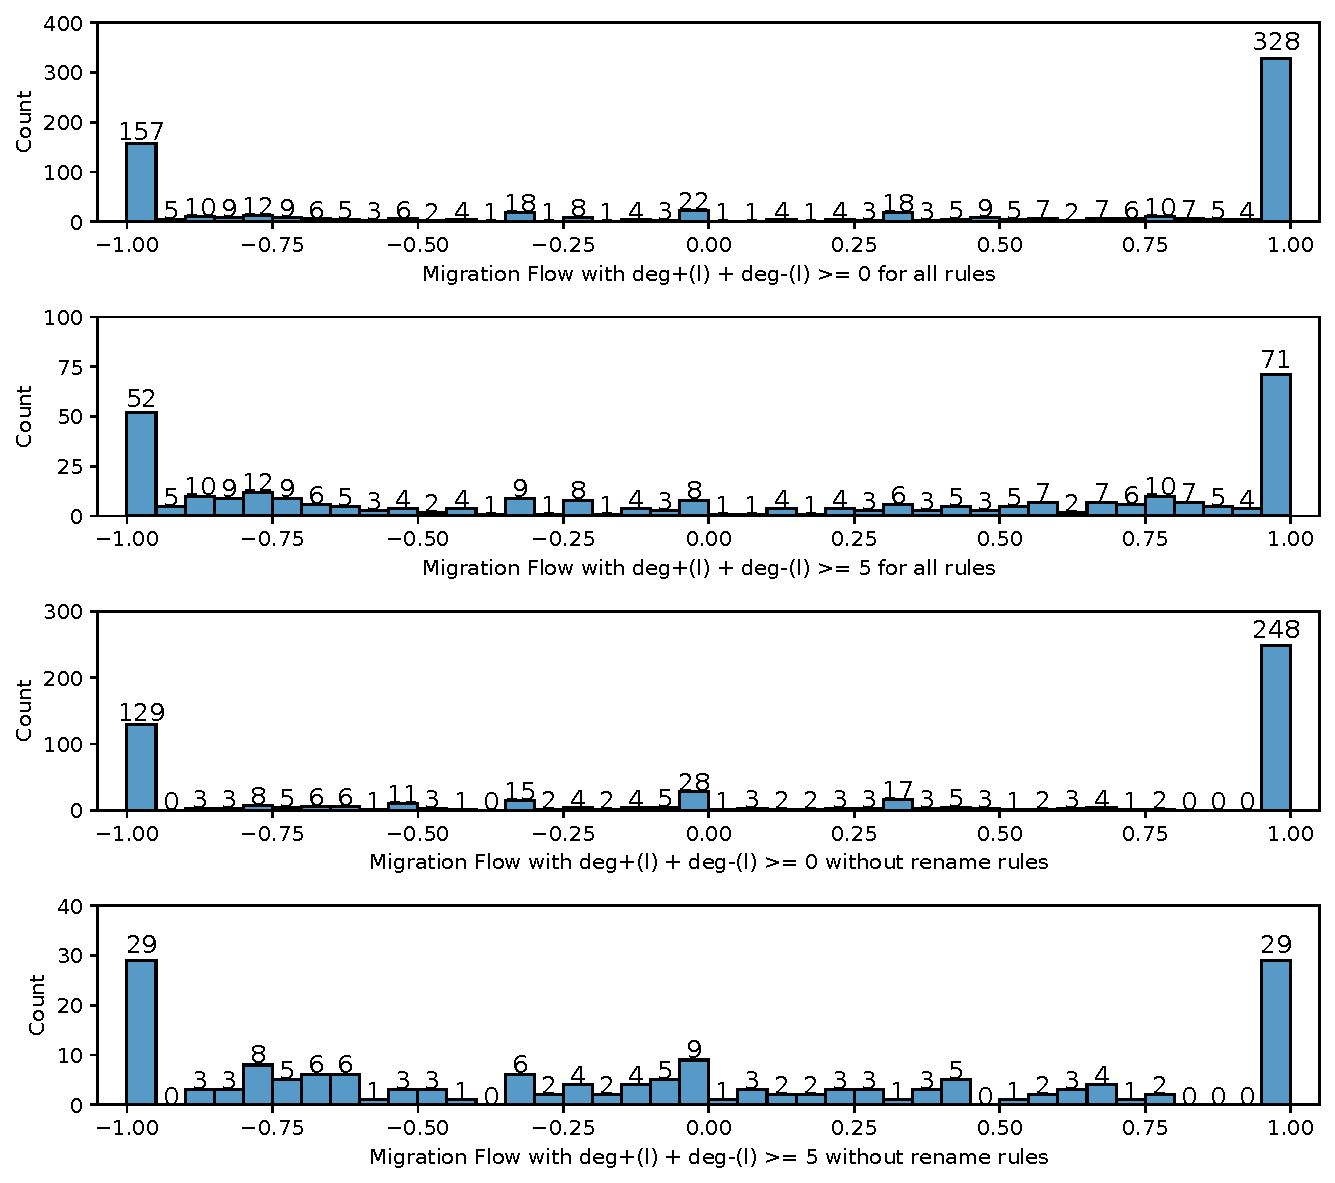
\includegraphics[width=\linewidth]{fig/flow.pdf}
  \vspace{-7mm}
  \caption{Distribution of $flow(l)$ under different conditions.}
  \label{fig:flow}
  \vspace{-4mm}
\end{figure}

\begin{comment}\begin{figure}
\begin{subfigure}[b]{\linewidth}
  \centering
  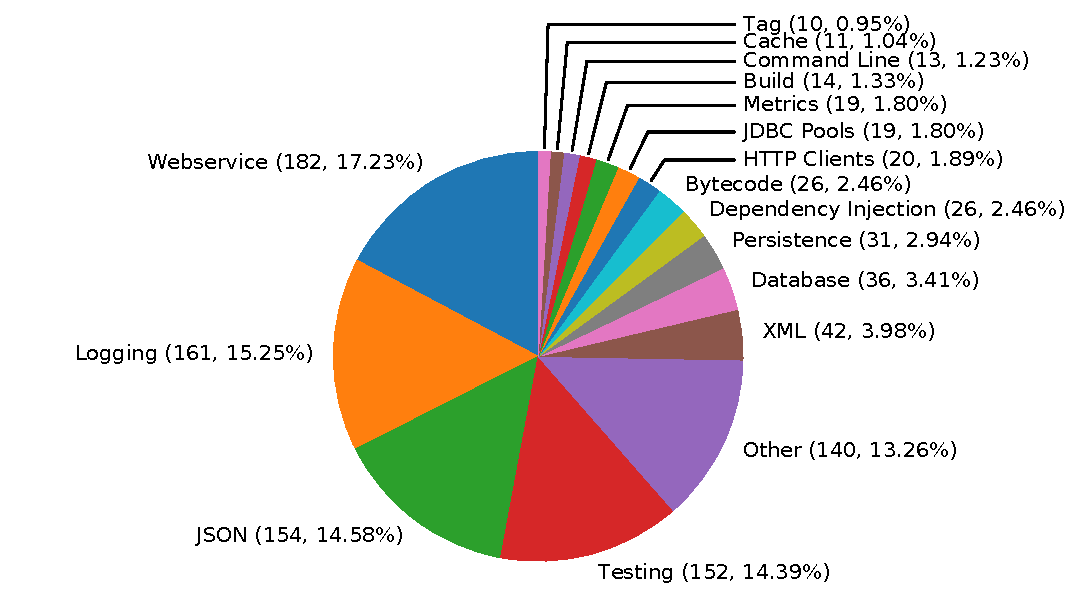
\includegraphics[width=\textwidth]{fig/migcat.pdf}
  \vspace{-2mm}
  \caption{Distribution of $\mathcal{R}$ by application domain.}
  \label{fig:migcat}
\end{subfigure}

\begin{subfigure}[b]{\linewidth}
  \centering
  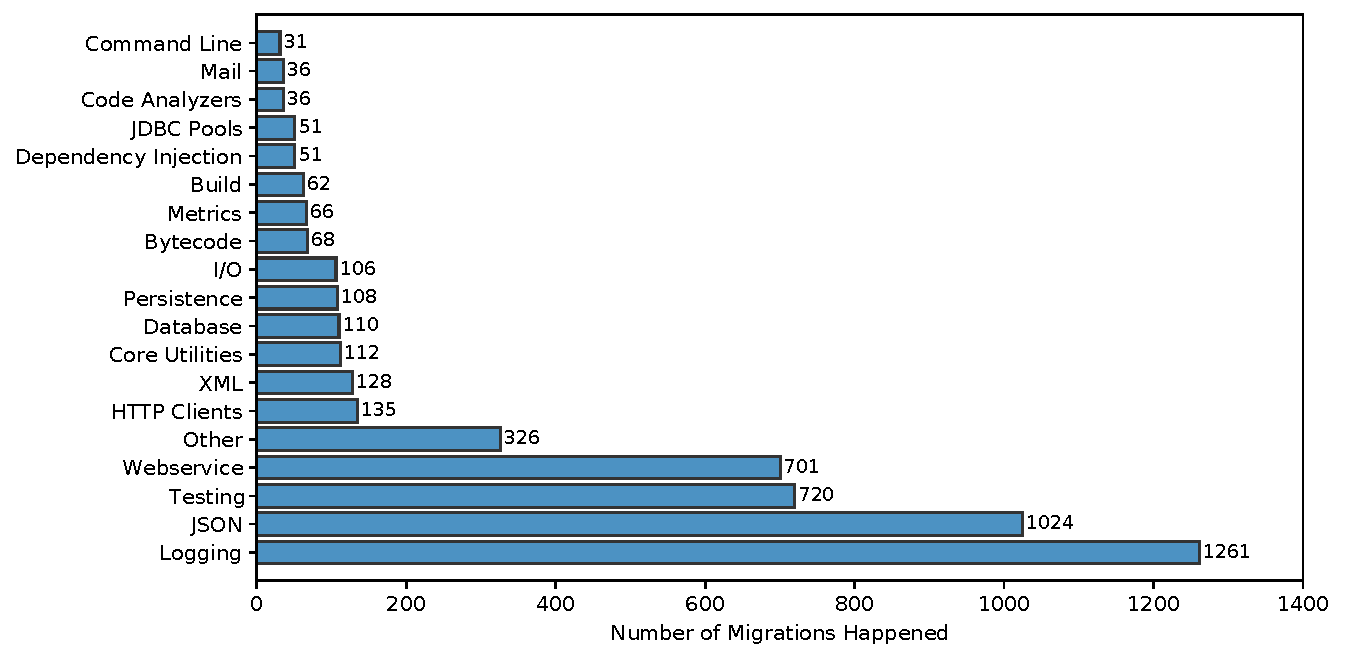
\includegraphics[width=\textwidth]{fig/migrepodist.pdf}
  \vspace{-2mm}
  \caption{Number of migrations happened for migration rules in each application domain ($\sum_{p\in \mathcal{P}} MigCnt(p)$, Equation \ref{eq:migcount}).}
  \label{fig:migrepodist}
\end{subfigure}

\begin{subfigure}[b]{\linewidth}
  \centering
  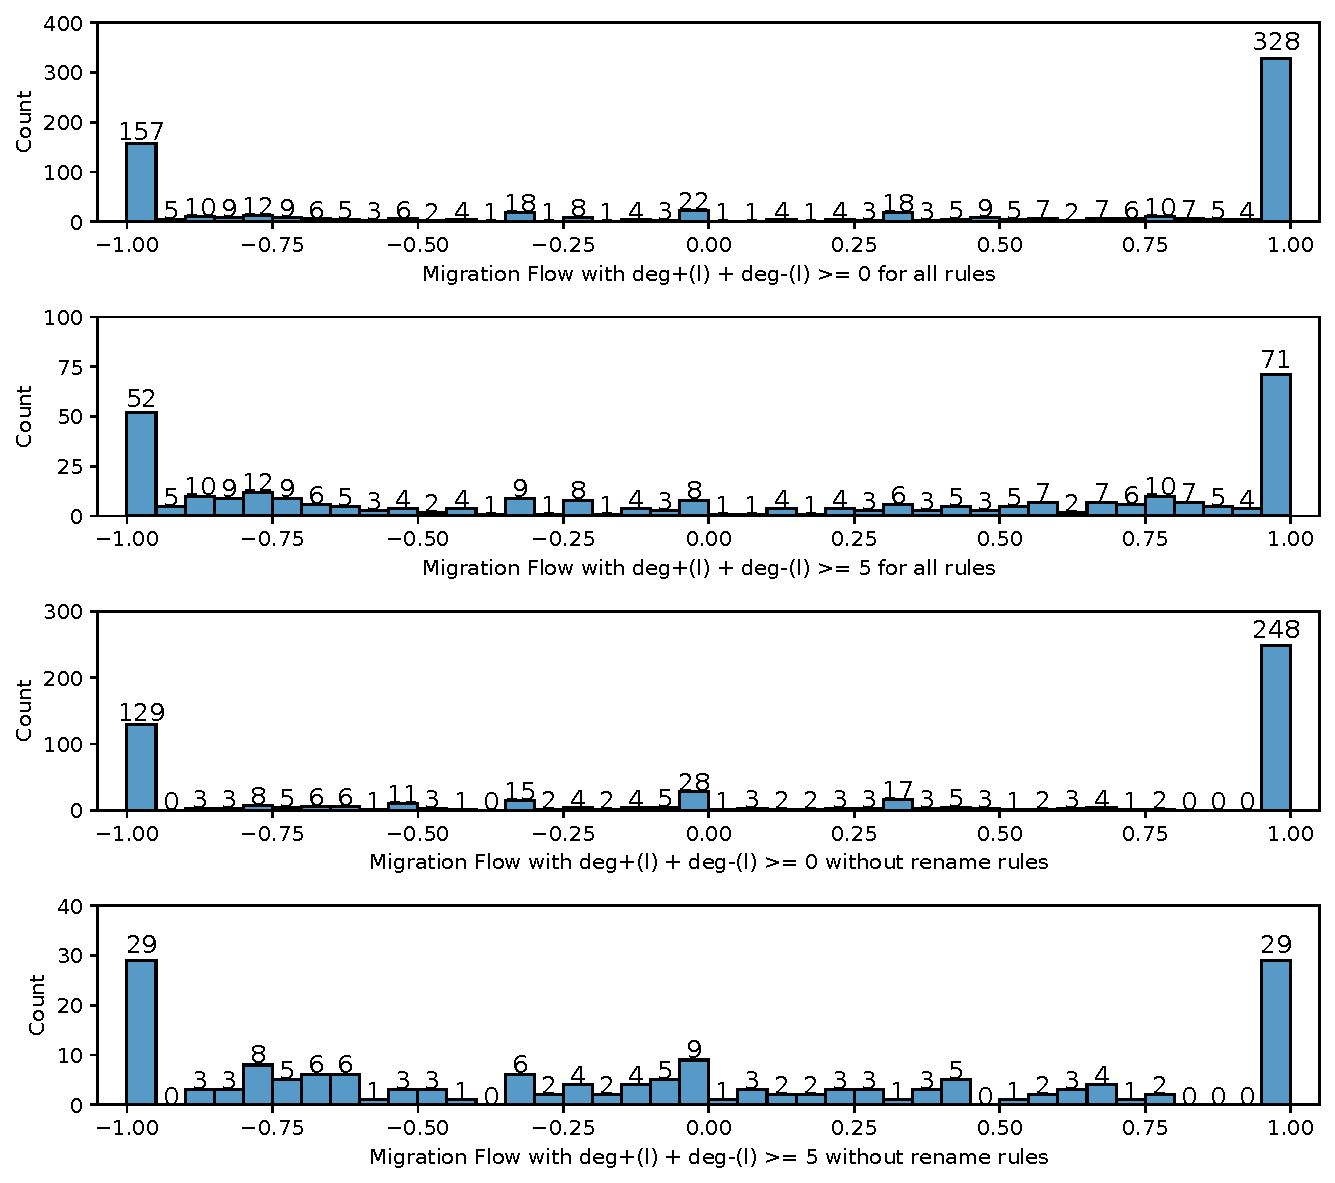
\includegraphics[width=\textwidth]{fig/flow.pdf}
  \vspace{-2mm}
  \caption{Distribution of $flow(l)$ under different conditions.}
  \label{fig:flow}
\end{subfigure}
\vspace{-2mm}
\caption{How migrations happen between libraries.}
\vspace{-4mm}
\end{figure}\end{comment}

\begin{figure*}[t]
  \centering
  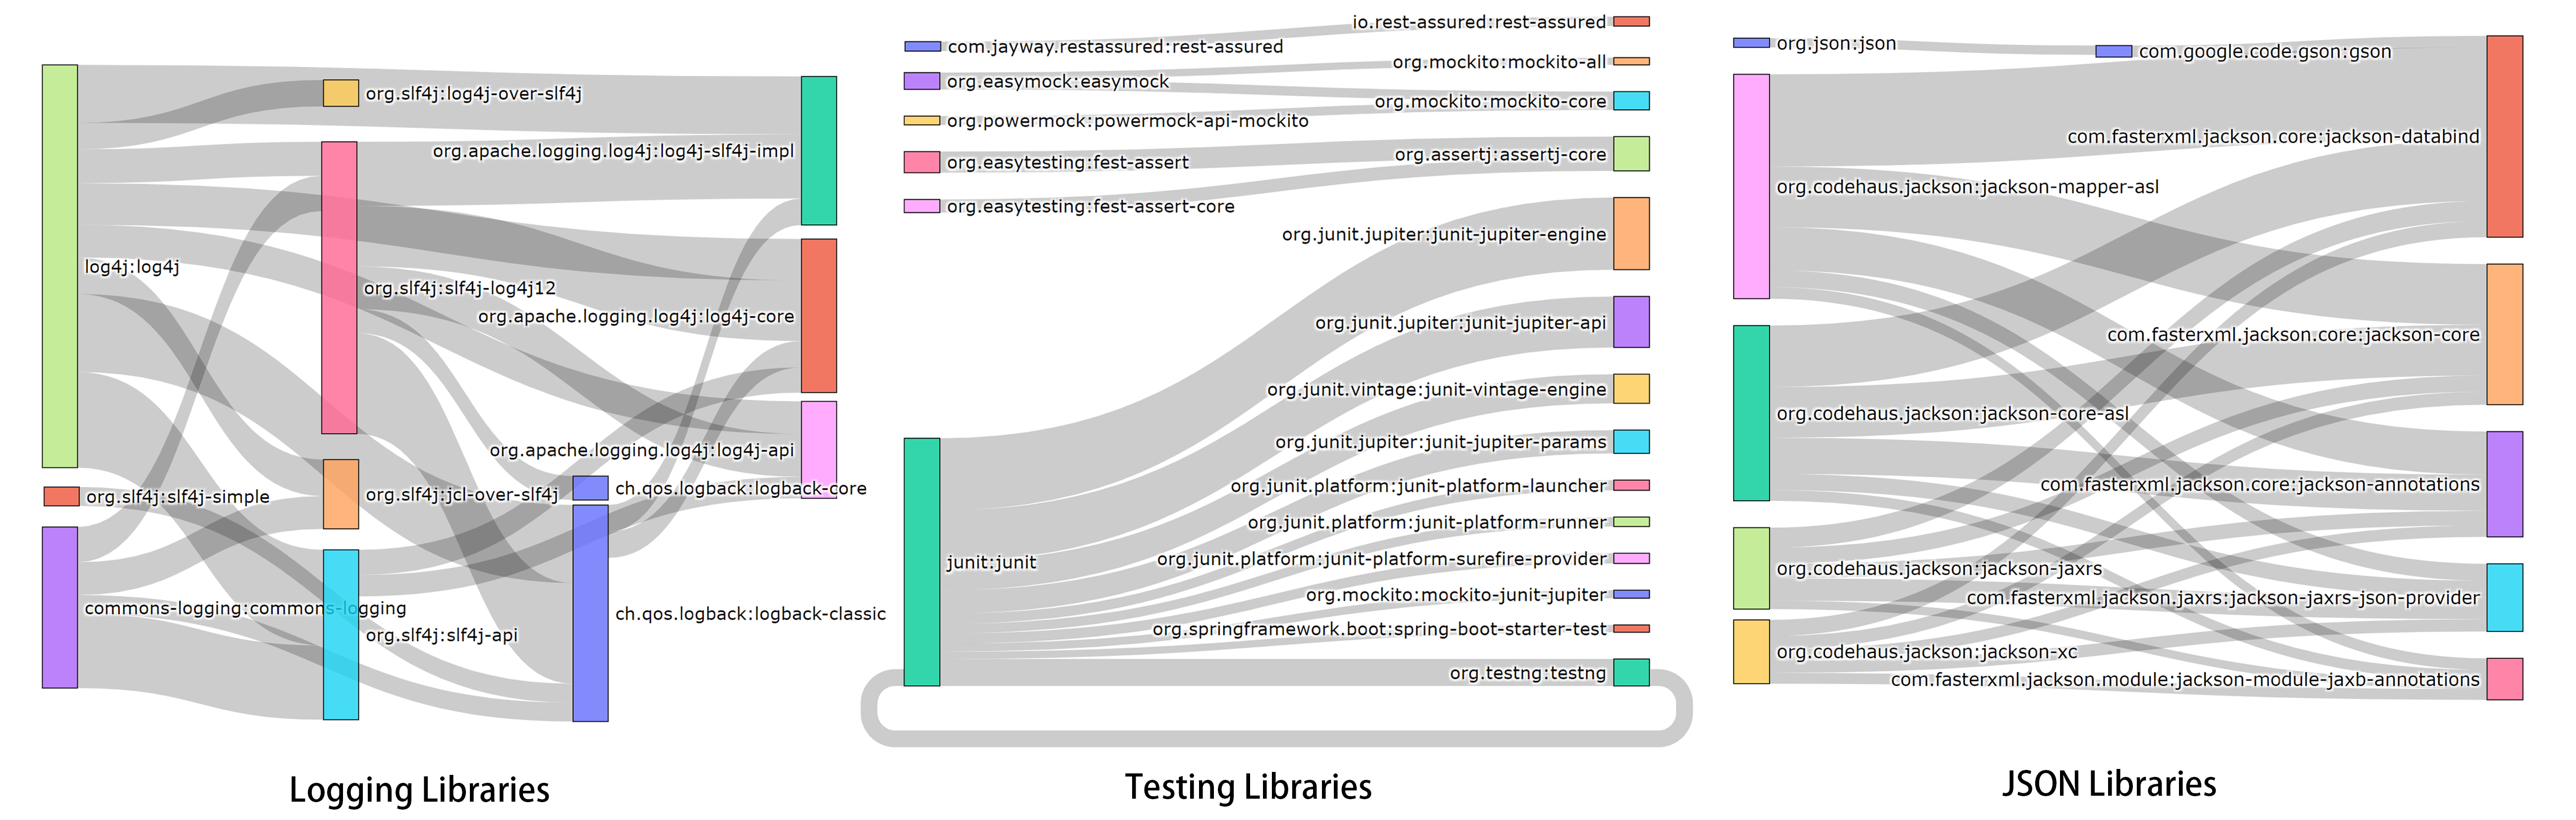
\includegraphics[width=\linewidth]{fig/graph.png}
  \vspace{-6mm}
  \caption{The migration sub-graphs for logging, testing, and JSON libraries. Migrations flow from left to right. Each rectangle is a graph node (i.e, library) and each grey band is a graph edge (i.e., migration rule). %and the rectangle height encodes its popularity (number of projects that adopted this library). 
  For each edge, its band width encodes the number of repositories where migrations happened for this migration rule.
  %The node color encodes its $flow(l)$, from red (-1) to green (1).  and its stroke width encodes its edge weight (number of projects where this migration happened).
  }
  \label{fig:miggraph}
  \vspace{-2mm}
\end{figure*}

Figure~\ref{fig:flow} (top) shows the distribution of $flow(l)$ for $l \in L_m$.
Surprisingly, the distribution is extremely distorted.
For 154 libraries (21.51\%), $flow(l) = -1$ and for 326 libraries (45.53\%), $flow(l) = 1$.
The remaining libraries generate a uniform distribution in the interval of $(-1, 1)$.
The distribution shape does not change even if we only consider libraries with higher indegree and outdegree values (Figure~\ref{fig:flow} second top), although there are slightly more libraries that fall within the interval of $(1, -0.75] \cup [0.75, 1)$.
The distribution shape also does not change even if rename rules are excluded (Figure~\ref{fig:flow} second bottom and bottom).
We can conclude from this observation that a large number of libraries are either mostly abandoned or mostly adopted as migration targets by developers, which indicates that some libraries are more competitive than others and should be recommended to use instead of the other libraries.

As illustrating examples, we visualize the sub-graphs of three most popular application domains (logging, testing, and JSON) in Figure~\ref{fig:miggraph}.
We exclude the sub-graph for web service due to space constraints.
To make the graphs readable, we only retain migration rules $\langle l_1, l_2 \rangle$ with $w(l_1, l_2) \ge 10$ for testing and JSON, and $w(l_1, l_2) \ge 15$ for logging.
The unidirectional trend is clearly visible using Sankey diagrams.
In the case of logging libraries, \Code{commons-logging}~\cite{commons-logging} and \Code{log4j}~\cite{log4j} are two mostly abandoned libraries, while libraries under group ID \Code{org.apache.logging.log4j}  (i.e., \Code{log4j} 2~\cite{log4j2}) are mostly adopted. 
Libraries related to \Code{slf4j}~\cite{slf4j} and \Code{logback}~\cite{logback} are somewhere in between.
The reason for such phenomenon may be that the Java community has two major logging practice changes~\cite{kabinna2016logging}: one is from ad-hoc logging libraries (e.g., \Code{log4j}) to logging abstraction libraries (e.g., \Code{slf4j}); another is from logging abstraction libraries to logging unification libraries (e.g., \Code{log4j} 2).
Such multiple paradigm shifts can also be observed in JSON libraries (e.g., \Code{gson}~\cite{gson} is first adopted but then switched to \Code{jackson}~\cite{jackson}), but not obvious in testing libraries.
%The majority of web service migrations is because of renames (due to major version updates), which may indicate that switching between different web service frameworks are too costly to perform.
We can also see that rename rules constitute a large number of migrations for testing and JSON (many non-rename rules are omitted in Figure ~\ref{fig:miggraph} because they happen in less than 10 projects).
In all cases, hardly can we see two libraries with major bi-directional flows, except the case of \Code{junit:junit}~\cite{junit4} and \Code{org.testng:testng}~\cite{testng}, which may be the results of early competition when both libraries are immature.
%but eventually, most projects choose \Code{junit5}~\cite{junit5} related libraries.

\begin{result-rq}{Summary for RQ2:}
Library migrations from four domains (logging, testing, JSON, and web service) among 53 dominate the dataset, presenting a long tail distribution.
Also, library migrations are highly unidirectional in that most libraries are either mostly adopted or mostly abandoned.
\end{result-rq}

\section{RQ3: What are the frequently mentioned reasons when developers conduct a library migration?}

RQ1 and RQ2 demonstrate \textit{how} library migrations happen in Java software projects, but it is still unclear \textit{why} library migrations happen in these projects.
Understanding the latter is important because we can extract retrospective insights for practitioners by summarizing the rationale behind previous migrations.
Therefore, we ask \textbf{RQ3:} What are the frequently mentioned reasons when developers conduct a library migration?

\subsection{Methodology}

To answer RQ3, we choose to study developer-written texts related to existing migrations.
We begin with the commit messages of the 3,340 migration commits ($\mathcal{M}$, Section~\ref{sec:get-lib-mig}).
To extend available data, we follow GitHub conventions to identify issue references in commit messages~\cite{github-issue-link}, and retrieve pull requests containing the commits using the GitHub RESTful APIs.
We get 2,775 pull requests and 385 issues after this step.
To extract reasons from these related texts, we follow the general procedure of thematic analysis~\cite{braun2012thematic, cruzes2011recommended}, which is frequently used to extract recurring patterns from text in software engineering research (e.g.,~\cite{silva2016we, coelho2017modern, tan2019communicate}).

Since a large amount of text in commit messages, issue/PR descriptions and comments are not relevant to migration reasons, three of the authors first independently read and re-read all text in the commits, issues and PRs to mark relevant text about migration reasons.
After the marks are merged and verified through discussion, we get 351 (10.51\%) commits, 223 (8.04\%) pull requests and 112 (33.53\%) issues that include some text stating the reasons for this migration.
The ratios are low either because developers just document what they have done instead of the rationale behind their work or because some issues and PRs are discussing other topics, but we still acquire the largest amount of data to answer this question compared with existing works~\cite{teyton2014study, kabinna2016logging} (Table~\ref{tab:related-work}).

Next, one author reads through all materials and generates 23 initial codes for migration reasons and a coding book that defines these codes.
Then, he and another author independently use the coding book to code all materials, in which each commit/issue/PR can be assigned multiple codes.
To deal with materials with more than one code, we use MASI distance~\cite{passonneau2006measuring} as the distance measure and Krippendorff's alpha~\cite{krippendorff2011computing} to measure inter-rater agreement. The first round of coding results in a Krippendorff's alpha of 0.731, which is lower than the recommended threshold of 0.8~\cite{krippendorff2018content}.
To reduce disagreement, we identify ambiguous codes and discuss solutions until a consensus is reached.
We decide to merge some of the ambiguous codes (e.g., ``ease of use'' and ``flexibility'' are merged into ``usability'') to generate final themes, and resolve the remaining conflicts after the merging.
Finally, the 23 codes are merged into 14 sub-themes organized into three themes (source library, target library, and project specific) and an additional ``other'' theme.
The Krippendorff's alpha of initial coding results after mapping to the 14 sub-themes is 0.803.
The main reason for most disagreements is that some text do not provide sufficient information for distinguishing between different sub-themes.
During the conflict resolution process, the two aforementioned authors first discuss about the relevant text content to see if anyone has misunderstandings or labeling mistakes.
If the text contains insufficient information or ambiguities, they may search over the Web, inspect the project development history, and infer the underlying reasons based on their prior experience.
One author has 4 years of Java development experience and arbitrates most of the cases.
Cases where the conflicts cannot be resolved will be simply labeled as ``other.''

\subsection{Results}

\begin{table*}
  \caption{Reasons for Library Migration. Reasons marked with $\dag$ are not mentioned in existing work on library migrations. We also extend and re-organize reasons mentioned in existing work (marked with $\S$).}
\vspace{-3mm}
  \label{tab:reason}
  \begin{tabular}{lrrl}
  \toprule
    Reason & Projects & Rename Rules & Top-4 Application Domains \\
    \midrule
    Source Library                     & 135 (32.14\%)  & 68/135 (50.37\%) & \Tag{Logging (23)}, \Tag{HTTP Clients (19)}, \Tag{Testing (16)}, \Tag{JSON (15)} \\%XML (11)\\
    \MyIndent Not Maintained/Outdated$^\S$  & 77  (18.33\%)  & 25/54 (46.30\%)  & \MyIndent \Tag{Testing (13)}, \Tag{Logging (10)}, \Tag{JSON (8)}, \Tag{HTTP Clients (8)} \\ %Core Utilities (4)\\
    \MyIndent Bug/Other Issue$^\S$         & 41  (9.76\%)   & 35/71 (49.30\%)  & \MyIndent \Tag{Logging (7)}, \Tag{XML (5)}, \Tag{Database (3)}, \Tag{HTTP Clients (3)} \\% Command Line (3)\\
    \MyIndent Security Vulnerability$^\dag$   & 26  (6.19\%)   & 27/40 (67.50\%)  & \MyIndent \Tag{HTTP Clients (9)}, \Tag{Logging (6)}, \Tag{JSON (5)}, \Tag{XML (5)}\\% Core Utilities (1)\\
    Target Library                     & 166 (39.52\%)  & 77/247 (31.17\%) & \Tag{Logging (55)}, \Tag{Testing (33)}, \Tag{JSON (14)}, \Tag{Web Service (11)}\\% Database (11)\\
    \MyIndent Usability$^\S$                & 76  (18.10\%)  & 20/95 (21.05\%)  & \MyIndent \Tag{Logging (35)}, \Tag{Testing (13)}, \Tag{Database (4)}, \Tag{JSON (3)}\\%, JDBC Pools (2)\\
    \MyIndent Feature                  & 57  (13.57\%)  & 53/125 (42.40\%) & \MyIndent \Tag{Testing (13)}, \Tag{Logging (9)}, \Tag{JSON (8)}, \Tag{Web Service (5)}\\%, Command Line (5)\\
    \MyIndent Performance             & 28  (6.67\%)   & 7/32 (21.88\%)   & \MyIndent \Tag{Logging (5)}, \Tag{Web Service (3)}, \Tag{Database (3)}, \Tag{HTTP Clients (2)}\\%, JSON (2)\\
    \MyIndent Size/Complexity$^\dag$          & 10  (2.38\%)   & 0/10 (0.00\%)    & \MyIndent \Tag{Logging (2)}, \Tag{JSON (1)}, \Tag{Database (1)}, \Tag{Bytecode (1)}\\%, HTTP Clients (1)\\
    \MyIndent Popularity$^\dag$               & 9   (2.14\%)   & 11/17 (64.71\%)  & \MyIndent \Tag{Testing (3)}, \Tag{Logging (2)}, \Tag{HTTP Clients (1)}, \Tag{I/O (1)}\\%, Web Service (1)\\
    \MyIndent Stability/Maturity$^\dag$      & 8   (1.90\%)   & 3/8 (37.50\%)    & \MyIndent \Tag{Logging (2)}, \Tag{Testing (2)}, \Tag{JDBC Pools (1)}, \Tag{Persistence (1)}\\
    \MyIndent Activity$^\dag$                & 6   (1.43\%)   & 0/5 (0.00\%)     & \MyIndent \Tag{Testing (2)}, \Tag{Reflection (2)}, \Tag{Classpath (2)}, \Tag{Code Analyzer (1)}\\%, Command Line (1)\\
    Project Specific                  & 188 (44.76\%)  & 77/247 (36.82\%) & \Tag{Logging (42)}, \Tag{JSON (24)}, \Tag{Testing (24)}, \Tag{Web Service (22)}\\%, XML (11) \\
    \MyIndent Integration$^\S$            & 125 (29.76\%)  & 90/207 (43.48\%) & \MyIndent \Tag{Logging (24)}, \Tag{Web Service (17)}, \Tag{Testing (16)}, \Tag{JSON (12)}\\%, Persistence (10) \\
    \MyIndent Simplification$^\S$          & 53  (12.62\%)  & 21/81 (25.93\%)  & \MyIndent \Tag{Logging (21)}, \Tag{Testing (9)}, \Tag{JSON (5)}, \Tag{Web Service (5)}\\%, Core Utilities (3) \\
    \MyIndent License$^\dag$                & 22  (5.24\%)   & 4/20 (20.00\%)   & \MyIndent \Tag{Code Analyzers (6)}, \Tag{JSON (6)}, \Tag{PDF (3)}, \Tag{Math (2)}\\%, Concurrency (2) \\
    \MyIndent Organization Influence$^\dag$   & 5   (1.19\%)   & 9/12 (75.00\%)   & \MyIndent \Tag{Command Line (2)}, \Tag{JSON (1)}, \Tag{Build (1)}, \Tag{XML (1)} \\
    Other                              & 21  (5.00\%)   & 24/42 (57.14\%)  & \Tag{JSON (6)}, \Tag{Logging (6)}, \Tag{Web Service (4)}, \Tag{Database (2)}\\%, Cache (1) \\
  \bottomrule
  \end{tabular}
\vspace{-3mm}
\end{table*}

We summarize 14 reasons for migration in Table~\ref{tab:reason} with three themes: 1) reasons originated from the \textit{source library}, 2) reasons motivated by the \textit{target library}, and 3) \textit{project specific} reasons.
To avoid duplication (i.e., multiple issues/PRs mentioning the same migration), we estimate the frequency of each reason by the number of projects that have a commit/issue/PR that mentioned this reason (420 projects in total).
We also show the proportion of rename rules among all rules and top-4 application domains by the aforementioned frequency for each reason.
Among the 14 reasons, 7 reasons (marked with $\dag$) are not discussed in existing work (Table~\ref{tab:related-work}), and 5 reasons (marked with $\S$) originate from existing work but are further extended and re-organized based on our findings.
In the remainder of this section, we will introduce each reason in detail.

\subsubsection{Source Library}

135 projects (32.15\%) conduct library migrations because of problems in the source library, with three dominating factors: the source library is not maintained/outdated, suffers from security vulnerabilities, or contains bugs/other issues.

\textbf{Not Maintained/Outdated.} 
The migration happens because the source library is old and/or lacks maintenance, and the project decides to use the library that is currently recommended and supported by the community.
It is the most common reason in source libraries for both rename rules and other rules. 
Examples: 1) \textit{Replace end of life apache http client 3.1 with 4.1}.\footnote{Commit \texttt{fa6f20b} in \url{https://github.com/basho/riak-java-client}}
2) \textit{FEST hasn't been updated in over 1 year. AssertJ looks like the successor}.\footnote{\url{https://github.com/dropwizard/dropwizard/issues/493}}
Teyton et al.~\cite{teyton2012mining} mention ``outdated'' as a reason for migration, but we further discover that the major concern is whether the library is still maintained, and the recognition of non-maintenance (e.g., announcement of end-of-life) often triggers migrations.

\textbf{Bug/Other Issues.}
The migration happens because of bugs, warnings, crashes, inconsistencies, unwanted features or other peculiar issues.
For example, \textit{Empty string is not working, when we pass ""...This seems to be a bug in jcommander}.\footnote{\url{https://github.com/ballerina-platform/ballerina-lang/issues/229}}

\textbf{Security Vulnerability.}
The migration happens because of security vulnerabilities in the source library, and also mostly because the source library does not provide any security fixes. 
This happens mostly for rename rules (67.50\%), and most notably for some of the migrations from \Code{log4j} to \Code{log4j} 2, \Code{slf4j} or \Code{logback}, e.g. \textit{Fix for log4j vulnerability CVE-2019-17571}.\footnote{\url{https://github.com/OpenLiberty/ci.maven/pull/717}}
It seems that security issue is the last straw that pushes these projects to finally abandon an old and unmaintained library.

\subsubsection{Target Library}
166 projects (39.52\%) conduct library migrations because of advantages in the target library.
Inspired by Larios Vargas et al.~\cite{larios2020selecting}, we divide them into the following 7 dimensions.

\textbf{Usability.} 
The most frequently mentioned reason in target library is that the target library is easy to use, has nice APIs, results in cleaner code, cleaner configuration, or is flexible for end users to switch implementations on need, e.g. \textit{allow users to use their preferred logging framework (such as logback) },\footnote{\url{https://github.com/apache/accumulo/pull/1163}} and \textit{Fest is awesome. The tests read better, and fest's fluent matchers are way easier to find (via auto-complete) than the static imported hamcrest matchers.}\footnote{Commit \texttt{05263e7} in \url{https://github.com/glowroot/glowroot}}
Some projects also mention that choosing an easy-to-use library is important for maintainability in the future.
Kabinna et al.~\cite{kabinna2016logging} mention ``flexibility'' and Teyton et al.~\cite{teyton2012mining} mention ``convenience'' as reasons for migration, but the former reason is specific to logging libraries (because many projects want to allow its downstream projects to switch underlying logger implementation on demand), and the latter term does not cover all the cases we find. 
Therefore, we decide to merge them into a broader sub-theme of ``usability.''

\textbf{Feature.}
A large number of migrations also happen because the target library has specific features that the source library cannot provide. 
For example, \textit{Use gson to preserve the order of all fields.}\footnote{\url{https://github.com/apache/incubator-pinot/pull/2473}}
The mentioned features are highly diverse across different application domains and project contexts. 

\textbf{Performance.}
Performance is also frequently mentioned as a reason for migration.
In most cases, the migration happens because a project needs to meet special functional requirements (e.g. latency, throughput, compile time, etc) that the existing library cannot satisfy.
For example, \textit{log4j has been identified as a
performance bottleneck for high qps use cases.}\footnote{\url{https://github.com/apache/incubator-pinot/pull/4139}}

\textbf{Size/Complexity.} 
Some projects care about the binary size or simplicity of the library, mostly because they want their own binary to be as small as possible, e.g.
\textit{ Swapped H2 database to Hypersonic SQL to make stubby4j JAR smaller}.\footnote{Commit \texttt{ce45e04} in \url{https://github.com/azagniotov/stubby4j}}

\textbf{Popularity.} 
Surprisingly, popularity is not a frequently mentioned reason, and most of the cases are because of library renames (64.71\%). It may be because it is too trivial to be mentioned or discussed, or because popularity alone does not provide immediate benefits and thus is not the decisive factor of a migration.

\textbf{Stability/Maturity.} 
A few projects mention that the target library is stable or more robust.
It may not be the decisive factor, but the factor that finally drives a migration, e.g., \textit{JUnit 5 will be available soon as a stable release. 
It is available a alpha/beta now.
As soon as it is available, all the unit tests may use this version.}\footnote{\url{https://github.com/sarl/sarl/issues/875}}

\textbf{Activity.}
A few projects mentioned the community is more active in the target library, but it is only mentioned along with other reasons (e.g. source library is not maintained) and never mentioned as the single decisive factor.

\subsubsection{Project Specific}
188 projects (44.76\%) mentioned that they conduct library migrations due to project specific reasons.

\textbf{Integration.} 
The most common reason is the need to integrate the library with something else in the project to achieve specific goals, avoid issues, or ensure compatibility.
We identify three major cases: 
1) to integrate with other dependencies to achieve a specific goal, e.g. utilize existing integration support, as stated in \textit{This change replaces the internal usage of Dropwizard in favor of Micrometer...This allows to take full advantage of the Spring Boot Micrometer integration.}\footnote{Commit \texttt{905e384} in \url{https://github.com/eclipse/hono/}}
2) to avoid conflicts / incompatibility with other dependencies or other project modules, e.g., \textit{Removes the PowerMock dependency which was having some bad interactions with Mockito.}\footnote{Commit \texttt{2aed070} in \url{https://github.com/GoogleCloudPlatform/java-docs-samples/}} 
3) to be compatible with the required runtime environment, e.g., \textit{migrate from lombok to kotlin...to a fix a bug with java 11.}\footnote{\url{https://github.com/spotify/ffwd/pull/140}}
Teyton et al.~\cite{teyton2014study} mention ``configuration'' and ``environment'', which we merge and extend into this sub-theme.

\textbf{Simplification.} 
Some migrations happen to simplify library usage within project, achieve consistent style, or cleanup unnecessary dependencies, as a preventive measure to control project complexity, remove technical debt, and possibly reduce maintenance effort in the future. 
For example, 1) \textit{Unify all JSON usage to fasterxml.jackson package. Remove the usage of json package from org.json, org.codehaus.jackson, com.google.code.gson, com.alibaba. Add JsonUtils class to reuse ObjectMapper and provide util methods}.\footnote{\url{https://github.com/apache/incubator-pinot/pull/3677}}
2) \textit{Make Logging Frameworks Coherent Across Libraries and IOT Codebase.}\footnote{Commit \texttt{dd5ae79} in \url{https://github.com/hortonworks/streamline/}}
3) \textit{Lots of cleanup. Removed Junit from a couple of modules (everything is TestNG now).}~\footnote{Commit \texttt{dfe5b79} in \url{https://github.com/dhanji/sitebricks}}
This sub-theme covers ``reduce the number of dependencies '' and ``reduce future maintenance'' mentioned in Kabinna et al.~\cite{kabinna2016logging}, and we further discover a frequent pattern in which many migrations happen because developers want to avoid using different libraries for the same purpose.

\textbf{License.}
For some projects and libraries, license compatibility stands out as the major reason for migration.
For example, 6 projects, including Spring Framework and Apache Hive, refrained from using \Code{org.json:json} because of its unusual license term \textit{The Software shall be used for Good, not Evil.}\footnote{\url{https://www.json.org/license.html}}
Other projects also migrate from various GPL or LGPL licensed libraries to other alternatives with more permissive licenses, such as Apache 2.0 and MIT.

\textbf{Organization Influence.}
Some projects remove a library because it is not approved by the belonging organization, or use a library as requested by the organization, e.g. \textit{Removes JLine2 as a dependency since it's not approved by LocationTech.}\footnote{Commit \texttt{833638f} in \url{https://github.com/locationtech/geogig/}}

\begin{result-rq}{Summary for RQ3:}
Projects conduct library migrations for 14 diverse reasons from the source library, the target library, and the projects themselves.
The most frequent reasons are: lack of maintenance in the source, feature / usability in the target, integration with project context, and simplification of dependencies.
\end{result-rq}

%\section{RQ4: Predictive Modelling}

%\subsection{Motivation}
%To validate our results and propose a model for practitioners, we propose to 

%\subsection{Methodology}

%\subsection{Results}

%\begin{result-rq}{Summary for RQ4:}
%a library is more likely to be adopted if ..., ..., and ..., %and more likely to be removed if ..., ..., and .... 
%\end{result-rq}

\section{Discussion}

% 只有在讨论Pracitioner实践,例如做推荐的时候,与哲学社会学有关的内容可以拎出来作为引用讨论,因此此段删去
\begin{comment}
\subsection{Technology Transition Theories}

In their theory of technology transition, library updates can be viewed as accumulated incremental innovations in stable regimes.

The theory of technology change by Rosenberg distinguish between the process of search and selection on the technological paradigms (e.g. library adoption and migration) and technical progress along a defined path (e.g. updates).

“A large portion of the total growth in productivity takes the form of a slow and often invisible
accretion of individually small improvements in innovations. (...) Such modifications are achieved by
unspectacular design and engineering activities, but
they constitute the substance of much productivity
improvement and increased consumer well-being in
industrial economies” (Rosenberg, 1982, p. 62).

``substitution of machines
for labour must be a powerful determinant
in the search process for new technologies.'' (Rosenberg, 1982, p9)

Keypoint: 
1) we can fit with the theory of Smith et al~\cite{smith2005governance}.
2) many complex mechanisms in the proposed theories remain unstudied.
3) some phenomenons in the theory cannot be observed for now, probably because most software is too young for such observation.

Smith et al. (2005) understand regime change to be
a function of two processes: (1) shifting selection pressures on the regime, (2) the coordination of resources
available inside and outside the regime to adapt to these
pressures. Selection pressures consist of economic pressures (competition, taxes, charges, regulations), broad
political, social and economic ‘landscape’ developments
(e.g. demographic shifts, rise of consumer culture, neoliberal model of globalisation) and pressures that “bubble
up from below, from innovative niches that are not yet
so established as to constitute a regime” (p. 1495). They
argue that “without at least some form of internal or
external pressure in the diverse senses discussed above,
it is unlikely that substantive change to the developmental trajectory of the regime will result” (p. 1495).
\end{comment}

\subsection{Takeaways for Practitioners}

\subsubsection{Best Practices}

Since our findings reveal that library migrations are highly unidirectional, it makes sense to formulate best practices on library migrations, and such best practices should be more publicly visible.
For example, package hosting platforms can compute and demonstrate the current retention rate for a library, as an additional metric to help developers decide whether to adopt or migrate the library.
Tools that help developers choose among a set of candidate libraries (e.g. AlternatveTo~\cite{AlternativeTo} and SimilarTech~\cite{chen2016similartech}) can make recommendations based on historical adoption, removal and migration trends.
Tools can also be developed to monitor the ``freshness'' of dependencies and prompt migration recommendations to developers based on the latest trends.

\subsubsection{Unmaintained Libraries}

Our findings also reveal that a large part of library migrations happen because of unmaintained libraries (Table~\ref{tab:reason}), and the situation significantly worsens if an unmaintained library has unfixed issues and security vulnerabilities.
However, open-source libraries are prone to sustainability failures~\cite{coelho2017modern, valiev2018ecosystem}, 
and unmaintained libraries may have vulnerabilities which may be even unknown to public but already discovered by malicious parties.
Given such risks, we suggest that software projects should \textit{refrain} from using an unmaintained library at all, and migrate to other alternatives as soon as possible.
However, determining whether a library is unmaintained may not be easy without community effort.
For example, we cannot easily tell whether a library is unmaintained from its last release time, because a mature library may not need to release frequently even if someone is still maintaining it.
Therefore, we also suggest package hosting platforms build a ``deprecation'' mechanism for their hosted libraries (similar to that of API).
Library maintainers can use this mechanism to announce their decision to no longer maintain a library, and package manager can automatically issue warnings to developers when they attempt to build their project with a ``deprecated'' library.
A similar deprecation mechanism is available in \Code{npm} for JavaScript libraries~\cite{cogo2021deprecation}, but not in Maven Central for Java libraries.

\subsubsection{Library Selection and Development}

We discover that among the library selection factors reported by Larios Vargas et al.~\cite{larios2020selecting}, only a few of them serve as the major driving pressure for library migration.
Most migrations happen because of usability, feature, or performance, and different application domains have different patterns (Table~\ref{tab:reason}).
Given that library migrations are generally costly~\cite{alrubaye2019use, chen2019mining}, it indicates that the gain in feature, performance or usability outweighs the costs, or the migration may be mission-critical and must be performed.
Therefore, we recommend developers to pay extra attention to these aspects and evaluate them with project requirements when selecting libraries, to avoid a costly migration in the future.
Library developers can also consider prioritizing their efforts on these aspects to make their library more competitive.

\subsubsection{Project Integration and Maintenance}

A large number of library migrations happen for integration with project context, simplification of dependencies, or license incompatibilities.
To prevent such migrations, we recommend project maintainers to check dependency conflicts or license incompatibilities before adopting a library, and avoid unnecessary dependencies (e.g., using different libraries for the same task).
Maintainers can use automated tools to facilitate these checks (e.g., \Code{maven-shade-plugin}, \Code{mvn dependency} commands, and open-source license checkers).
However, existing tools may be unable to check complex interaction issues or recommend best co-usage practices.
For example, one developer states in an issue that \textit{Spark really wants you to use log4j},\footnote{\url{https://github.com/openzipkin-attic/zipkin-sparkstreaming/issues/30}} but it is not obvious from Spark documentation.
Therefore, we also suggest library developers, especially framework developers, should explicitly document what libraries are recommended to use together with their library and what libraries are not recommended.
Researchers may also consider developing automated tools to alleviate this issue, e.g., by applying existing library recommendation approaches~\cite{thung2013automated, saied2018improving, nguyen2020crossrec} to discover co-usage patterns, or design new approaches to detect common integration pitfalls.

\subsection{Threats to Validity}
\label{sec:threat-to-validity}

\subsubsection{Internal Validity}
Extracting dependencies from \Code{pom.xml}s is the standard practice by many recent studies (e.g.,~\cite{cox2015measuring, dietrich2019dependency, kula2018developers, wang2020empirical}), but it comes with a number of limitations.
First, the declared dependencies may not be actually used (i.e., bloated) and used dependencies may be transitively included and not explicitly declared~\cite{soto2021comprehensive}. %, which means some removals will not be detected and we may underestimate the number of removals and the frequency of migrations.
Second, in multi-module projects, dependencies may be moved between different modules, which may cause over-estimations on removals and adoptions.
Our approach for computing dependency changes may also generate errors in some corner cases (e.g., a merge commit contains conflict resolution or is squashed with its parents~\cite{GitSquashMerge}).
All these cases will induce noises into our collected dependency changes and affect the results in RQ1, but they are generally recognized as bad practice and should not be very common in well maintained projects.
Additionally, we use self-admitted commit messages as the final criteria to ensure that all migrations we use to answer RQ2 and RQ3 are real migrations.
% However, dependency management files such as \Code{pom.xml}s are becoming increasing popular, recognized as best practice, and relied upon by many recent studies .
%2) in multi-module projects, dependencies may be moved between different modules, which may cause over-estimations on removals and adoptions. Such cases are hard to detect but should also be occasional and the noise should be minor.
%and may be undetectable because the histories in \Code{git} can be arbitrarily modified without leaving any remote traces~\cite{bird2009promises}.
For the collected library migrations, we do not know how complete or representative they are for all migrations in the wild.
However, projects with good commit messages about library migration may be of better quality than those without, so their practices should be more valuable for reference by other practitioners.
The manual identification of migrations, the resolution of application domains, and the thematic analysis process may all contain labeling errors.
To mitigate this threat, at least two authors double check the results for the first two steps and conduct independent coding for the thematic analysis.

\subsubsection{External Validity}
Our findings may not generalize to migrations that happen without being mentioned in commit messages and migrations in other projects and between other libraries.
We mitigate this threat by collecting a large number of starred GitHub projects and library migrations for popular libraries.
Our findings may also not generalize to projects that do not use build automation tools or projects that use other build automation tools (e.g., Gradle~\cite{gradle}), but Maven is the most popular tool~\cite{jvm-ecosystem-report} and the choice of automation tools should not significantly affect project properties,
Therefore, we believe our results will be useful for a broad audience of Java practitioners.
Finally, our results may not generalize to proprietary projects and projects in other programming languages / ecosystems (e.g., JavaScript/npm, Python/PyPI, etc). 
Intuitively, the results may differ because of difference in application domain, developer preferences, and stakeholder interest, and we leave the investigation of ecosystem differences as future work.

\section{Conclusion and Future Work}

In this paper, we conduct a descriptive mixed methods study on \textit{how} and \textit{why} library migrations happen in Java software projects. %based on the largest dataset to-date in the topic of library migration. 
Our contributions are %
1) A framework for quantifying dependency changes and library migrations based on version control data.
2) Findings regarding prevalence, trends and rationales of library migration in Java projects.
3) A largest dataset to-date in the topic of library migration.
%1) a framework for quantifying library migrations from the perspective of prevalence, trends and rationales based on large-scale dataset, and 2) 7 new migration reasons not discussed in previous work.
% The main findings are: 1) library migrations are prevalent in large projects, 2) they mostly happen unidirectionally, and 3) they happen for 14 diverse library-side and project specific reasons.
%mainly because lack of maintenance in the source library, feature and usability in the target library, integration with project context, and simplification of dependencies.
%We also identify 7 reasons not discussed in previous work.
As future work, we plan to understand the decision-making process of library migration, and evaluate the practicality of existing automated approaches for library migration.

\begin{acks}
This work is supported by the National Key R\&D Program of China Grant 2018YFB1004201 and the National Natural Science Foundation of China Grant 61825201. 
We would also like to thank the anonymous reviewers for their constructive feedback.
\end{acks}

\bibliographystyle{ACM-Reference-Format}
\bibliography{references}
\balance
\end{document}
\endinput
